\chapter{Network-based Wavelet Smoothing for Analysis of Genomic Data}
\label{chap:wavelet}

\begin{chapabstract}

\textrm{{\bf Abstract:}} Biological networks are a common way of describing information on relationships between genes that are accumulated from many years of biomedical research, and they are thus potentially valuable when incorporated as prior knowledge to guide biomarker selection in genomic data analysis. In this chapter, we focus on network-based regularization methods through a predictive framework with linear models, and propose to use a class of methods based on wavelet smoothing over undirected graphs that directly detect subnetworks composing of collaboratively functional gene modules. We perform breast cancer survival analysis using a large gene expression dataset and a protein-protein interaction network obtained from public database, and demonstrate that the proposed methods are able to improve the efficacy of gene selection in terms of stability, connectivity and interpretability while achieving competitive performance of survival risk prediction. Our results also serve a comparative study benchmarking several network-free and network-based regularization methods for gene selection related to breast cancer survival. This study is under preparation for submission as joint work with Jean-Philippe Vert \cite{Jiao2017Network}.
\linebreak
\vskip 0.1in
\noindent \textrm{{\bf R�sum�:}} 

\end{chapabstract}



\section{Introduction}
\label{sec3:introduction}






Genomic data analysis is a rapidly developing research area that receives increasing attention, thanks to the recent advancement of technologies in gene expression profiling that monitors the activity of a large number of genes in a single experiment. Identifying genes related to a clinical phenotype of interest, such as drug resistance or disease progression, is a central yet challenging topic in genomic research commonly known as biomarker selection. A typical approach follows a predictive framework that builds a predictive model linking genomic data to a clinical outcome further combined with a regularization method for feature selection and to address the high-dimensionality of high-throughput genomic data. For example, linear regression can be used to model the relationship between the quantitative measurements of toxicity response to a drug and the expression levels of all genes, and many regularization methods have been proposed in literature for identifying a few genes that are potentially related to the targets of the drug, including the well-studied and widely-used lasso \cite{Tibshirani1996Regression} and elastic net \cite{Zou2005Regularization}.







Despite the usefulness of the lasso-type regularization methods, the genes selected purely by such algorithmic approaches often lack proper mechanistic interpretation in terms of biological relevance and it remains a demanding task to determine \textit{a posteriori} whether and how the selected genes cooperate in some biological process. In fact, plentiful information about the interaction between gene products and the underlying biological functions is accumulated from extensive biomedical research over the years and can be obtained through many publicly available databases, including Human Protein Reference Database (HPRD) \cite{KeshavaPrasad2009Human}, Gene Ontology (GO) \cite{Ashburner2000Gene} and Kyoto Encyclopedia of Genes and Genomes (KEGG) \cite{Kanehisa2000KEGG}. Although these databases can help verify the collaborative functionality of a list of selected genes, the interpretation is usually non-trivial as many selected genes may seem unrelated or even unreliable.







To overcome the difficulty of \textit{a posteriori} interpretation of selected genes, there is therefore a need to develop methods that integrate prior knowledge in the process of biomarker detection in genomic data analysis in order to promote biological relevance. Although various databases register different aspects of interaction between gene products, this information is usually provided in the form of biological networks, which can be represented by graphs where vertices are genes and edges indicate some notion of interaction between the gene products of connected vertices. It has been demonstrated that genes closer on the network are more likely to be involved in similar biological functions and vice versa (see, e.g. \cite{Stuart2003gene}). The incorporation of biological networks to enhance biomarker selection consequently follows the principle that genes closer on the network should tend to be selected simultaneously. Note that this research topic is commonly phrased as \textit{network-guided biomarker discovery}, for which we refer to a tutorial-oriented survey by \cite{Azencott2016Network}.







In particular, we are interested in network-guided feature selection under a predictive framework via regularization methods. This network-based regularization should encourage that genes closer on the network contribute similarly to the predictive model built for some clinical phenotype and then, if selected, tend to be selected simultaneously. Notably, Laplacian regularization (Section \ref{sec3:fourier}) is a classic method that attempts to encourage smoothness between the coefficients of a linear model corresponding to neighboring features on the given network \cite{Belkin2004Regularization} but the regularization itself does not enforce sparsity nor enable feature selection. \cite{Li2008Network} proposed to combine sparsity-inducing penalties such as lasso with the Laplacian regularization for network-constrained feature selection with an application in genomic data analysis, and is further generalized in an adaptive fashion by \cite{Li2010Variable}. Besides Laplacian-based methods, many others stem from extending the standard lasso to structured regularization for identifying genes by groups. If meaningful gene groups can be defined by known functional gene modules on the network for instance, Group lasso \cite{Jacob2009Group,Yuan2006Model} can be used to force that genes belonging to the same groups are selected or disregarded simultaneously. Graph fused lasso \cite{Tibshirani2005Sparsity} encourages that the direct neighboring genes on the network share the same coefficients in a linear model, leading to the a partition of the network into subnetworks as functional gene modules. Pairwise $L_\gamma$ penalty \cite{Pan2010Incorporating} aims to model the instinct that direct neighboring genes in a network should be more likely to participate in the same biological process and thus tend to be selected simultaneously. Note that Laplacian regularization, which is intended for global smoothness, and group lasso, which is designed for group-wise gene signature selection, can also be combined \cite{Tian2013Network}.









We propose in this study to use a class of regularization methods for network-guided feature selection under a predictive modeling framework that simultaneously enjoy global smoothness over the network and directly identify subnetworks consisting of a few connected features. In fact, since the Laplacian regularization is known to be equivalent to a quadratic penalty with respect to the graph spectral domain \cite{Belkin2004Regularization}, the method essentially performs a graph Fourier transform on the coefficients of the linear models and then attenuates the high-frequency components thereof, therefore inducing global smoothness for the predictive models. A wealth of studies in the field of signal processing have been devoted to extending Fourier smoothing in order to simultaneously achieve spatial-temporal sparse coding, a topic that has been well established for data of regular structure such as time series or images \cite{Mallat1999wavelet} and has attracted much attention for data residing on irregular structure such as general graphs or manifolds \cite{Shuman2013emerging}. Following this trend, we propose to study network-based wavelet smoothing with an application to gemonic data analysis. Notably, when applied to biological networks, the global smoothness as well as localization properties of the network-based wavelet smoothing estimates a predictive model that directly enables the detection of subnetworks readily translated into functional gene modules, rendering interpretable biological insights concerning the particular phenotype of interest.










The chapter is organized as follows. In Section \ref{sec3:methods} we first elaborate the predictive modeling framework with regularization, with a particular emphasis on reviewing the network-based methods in literature, and then propose to use a class of novel methods based on wavelet smoothing on graphs. In Section \ref{sec3:results}, we perform simulated experiments and breast cancer survival analysis with gene expression data guided by a protein-protein interaction (PPI) network obtained from HPRD database. Promising results demonstrate the usefulness of the proposed methods for biomarker selection related to breast cancer survival, while they serve a comparative study benchmarking several methods of network-free and network-guided biomarker selection. All numerical experiments are implemented in \texttt{R} and codes and additional results are available via the online supplements found at \url{https://github.com/YunlongJiao/graphwavelet}. Finally we conclude and discuss in Section \ref{sec3:discussion}.









\section{Methods}
\label{sec3:methods}

\subsection{Feature Selection Under Predictive Modeling Framework}
\label{sec3:framework}



In supervised learning, let $\mathcal{D}:=\{(\xb_i,y_i):i=1,\dots,m\}$ denote a dataset of $m$ observations where each $\xb_i \in \RR^n$ is an $n$-dimensional feature vector that is paired with a quantitative measurement of some clinical phenotype $y_i$ to predict depending on the particular application. For instance, the feature values in $\xb_i = (x_{i1},\dots,x_{in})^\top$ can denote the expression levels of $n$ genes of sample $i$, while the quantity of the clinical phenotype can be a response $y_i \in \RR$ measuring the resistance to a drug of the sample, or a binary label $y_i \in \{-1,+1\}$ denoting whether a specific treatment is applied to the cancer patient, or a right-censored survival time $y_i=(T_i, \Delta_i) \in \RR \times \{0,1\}$ where, for some predetermined censoring time $C$, $(T_i|\Delta_i = 1)$ denotes the observed survival time of the diseased patient prior to $C$ or $(T_i|\Delta_i = 0)$ is equal to the censoring time $C$ meaning that the information is censored. Typically in biomedical applications, the number of genes is usually larger than the number of observations, i.e., $n > m$ or even $n \gg m$. We further assume that the feature data are standardized to have zero mean and unit variance, i.e., $\sum_{i=1}^m x_{ij}/m = 0$ and $\sum_{i=1}^m x_{ij}^2/(m-1) = 1$ for $j = 1,\dots,n$.








We consider linear models in this study where the quantity $y$ is linked with the underlying feature vector $\xb$ via a linear combination $\beta^\top \xb$ for some coefficient vector $\beta \in \RR^n$. For simplicity of notations, we do not consider intercepts explicitly in the discussion, but it can be easily included in the model by augmenting the feature vector with a dummy variable that takes constant value $1$. Given the dataset $\mathcal{D}$, an empirical procedure to estimate the coefficients $\beta$ is by solving optimization problems of the form:
\begin{equation}\label{eq3:glm}
\min_{\beta \in \RR^n} \ell(y_1, \dots, y_m, \beta^\top \xb_1, \dots, \beta^\top \xb_m) \,,
\end{equation}
where $\ell$ is a loss function measuring the empirical cost on the training data and should be carefully designed for specific application. For example, when $y_i \in \RR$ and
\begin{equation}\label{eq3:regression}
\ell(y_1, \dots, y_m, \beta^\top \xb_1, \dots, \beta^\top \xb_m) = \frac{1}{m} \sum_{i=1}^m (y_i - \beta^\top \xb_i)^2 \,,
\end{equation}
it recovers linear regression and returns the least squares solution; when $y_i \in \{-1,+1\}$ and 
\begin{equation}\label{eq3:classification}
\ell(y_1, \dots, y_m, \beta^\top \xb_1, \dots, \beta^\top \xb_m) = \frac{1}{m} \sum_{i=1}^m \log(1 + \exp(-y_i \beta^\top \xb_i)) \,,
\end{equation}
it recovers logistic regression for binary classification; when $y_i = (T_i, \Delta_i) \in \RR \times \{0,1\}$ and 
\begin{equation}\label{eq3:survival}
\ell(y_1, \dots, y_m, \beta^\top \xb_1, \dots, \beta^\top \xb_m) = -\frac{1}{m} \sum_{i=1}^m \Delta_i \{\beta^\top \xb_i - \log(\sum_{j:T_j>T_i} \exp(\beta^\top \xb_j))\} \,,
\end{equation}
it recovers the Cox proportional hazards model for survival analysis \cite{Cox1972Regression}. We would like to point out that the choice of the loss function is mostly application-oriented and is primarily not the concern of this study. In particular, the following discussion and our proposed methods will not depend on the choice of the loss function.








In order to avoid overfitting or to enable feature selection, it is usually suggested to incorporate appropriate regularization in \eqref{eq3:glm}. Specifically, we aim to solve optimization problems of the form:
\begin{equation}\label{eq3:regglm}
\min_{\beta \in \RR^n} \ell(y_1, \dots, y_m, \beta^\top \xb_1, \dots, \beta^\top \xb_m) + \lambda P(\beta) \,,
\end{equation}
where $P$ is a penalty term, especially one that induces sparsity for feature selection, and $\lambda \geq 0$ is a regularization parameter that trades off between the loss term and the penalty term. Classic penalty terms include the \textit{ridge} \cite{Hoerl1970Ridge} which penalizes the squared $L_2$ norm of the coefficient vector, i.e.,
\begin{equation}\label{eq3:ridge}
P^{\mbox{ridge}}(\beta) = \|\beta\|_2^2 \,.
\end{equation}
It is well-known that the ridge regularization is a shrinkage method that usually yields more robust estimate but does not enable feature selection. The \textit{lasso} \cite{Tibshirani1996Regression} is probably the simplest and most widely used sparsity-inducing regularization method which penalizes the $L_1$ norm of the coefficient vector, i.e.,
\begin{equation}\label{eq3:lasso}
P^{\mbox{lasso}}(\beta) = \|\beta\|_1 \,.
\end{equation}
The lasso enables feature selection by allowing a few non-zero coefficients in the estimate of $\beta$. Another widely used penalty extends the lasso by penalizing a weighted sum of the $L_1$ norm and squared $L_2$ norm on the coefficient vector that leads to a regularization method called \textit{elastic net} \cite{Zou2005Regularization}, i.e.,
\begin{equation}\label{eq3:enet}
P^{\mbox{e-net}}(\beta; \nu) = \nu \|\beta\|_1 + (1-\nu) \frac{1}{2} \|\beta\|_2^2 \,,
\end{equation}
where $0 \leq \nu \leq 1$ is a regularization parameter balacing between the two norms. In particular, the elastic net regularization reduces to the ridge when $\nu = 0$, and enables feature selection for $0 < \nu \leq 1$ including as a special case the lasso when $\nu = 1$. Despite that the elastic net regularization usually helps produce more reliable solutions when applied to biomedical data, the selected genes corresponding to non-zero coefficients often give no clear biological meaning in terms of their collaborative functionality. One possible solution is to devise a $L_{2,1}$ mixed norm, often termed as \textit{group lasso} \cite{Yuan2006Model, Jacob2009Group}, to force that eventually certain genes that belong to the same group, if selected, will be selected simultaneously. The groups of genes are defined \textit{a priori} by external knowledge. For example, genes that belong to the same pathway or contribute to the same biological process can be grouped together. However, as most biomedical databases provide domain-specific knowledge on gene interactions in the form of biological networks, we are interested in directly exploiting the network structure in order to guide biomarker selection.








\subsection{Network-guided Feature Selection: An Overview of Related Work}
\label{sec3:fourier}





Suppose a network that specifies the relationships between features is represented by an undirected weighted graph $\GG = (\VV, \EEc, A)$, where $\VV$ denotes the set of vertices representing the $n$ features indexed by $\{1,\dots,n\}$, $\EEc \subset \VV \times \VV$ denotes the set of edges with $(u, v) \in \EEc$ representing a link between vertices $u$ and $v$, $A \in \RR^{n \times n}$ is the weighted adjacency matrix such that $A_{uv} = A_{vu} =: a(u,v)$ with $a(u,v) > 0$ the weight assigned to an edge $(u,v) \in \EEc$ and $a(u,v) = 0$ if $(u,v) \notin \EEc$. In particular, we assume that no self-loop exists, i.e., $(u,u) \notin \EEc$ for any vertex $u$. Depending on the network under consideration, the weighted edges can be used to register the uncertainty of the existence of a link or the strength of the interaction between connected vertices.






Recall that a common assumption for network-guided feature selection under predictive framework is that we would like to devise penalty terms that encourage the coefficients corresponding to those features closer on the network to be similar so that, if selected, they tend to be selected together. To this end, let us first define the graph Laplacian $L = D - A$ where $D$ is a diagonal matrix with $D_{uu} = \sum_{v \neq u} a(u,v) =: d(u)$ the degree of the vertex $u$, i.e.,
\begin{equation*}
L_{uv} = \left\{
\begin{array}{ll}
d(u) & \mbox{if } u = v, \\
-a(u,v) & \mbox{if } (u,v) \in \EEc, \\
0 & \mbox{otherwise.}
\end{array}
\right.
\end{equation*}
The graph Laplacian is a key concept in spectral graph theory that shares many properties with the Laplace operator on Riemannian manifolds and reflects many properties of the graph structure \cite{Chung1997Spectral}. For example, $L$ is a symmetric, positive semi-definite matrix whose number of zero eigenvalues is equal to the number of maximally connected components of the graph. Note that some authors prefer to use alternatively the \textit{normalized} graph Laplacian defined as $\mathcal{L} = D^{-\frac{1}{2}} L D^{-\frac{1}{2}}$, particularly accounting for the degrees of different vertices. While the discussion in this study does not depend on which version of Laplacian (normalized or non-normalized) is used, they usually give very different results in practice as we will empirically demonstrate in Section \ref{sec3:results}. An important observation regarding the graph Laplacian is that it can be used to define measure of smoothness with respect to the graph structure for any vector whose covariates naturally reside on the vertices of the graph. We define the penalty term for \textit{Laplacian regularization} as
\begin{equation}\label{eq3:laplacian}
P^{\mbox{lap}}(\beta) = \beta^\top L \beta = \sum_{(u,v) \in \EEc} (\beta_u - \beta_v)^2 a(u,v) \,.
\end{equation}
In words, the Laplacian regularization method ``shrinks'' the pairwise difference between neighboring features to be small taking into account the edge weights and hence encourages solutions to be smooth over the graph.







It is very interesting to understand how the Laplacian regularization \eqref{eq3:laplacian} achieves global smoothness from a spectral perspective. As $L \in \RR^{n \times n}$ is symmetric and semi-positive, we have the eigendecomposition
$$
L = X \Lambda X^\top
$$
for an orthogonal matrix $X = (\chi_1 | \dots | \chi_n)$ where $\chi_i$ denotes the $i$-th column of $X$ and a diagonal matrix $\Lambda = \mbox{diag}(\lambda_1,\dots,\lambda_n)$ with $0 = \lambda_1 \leq \dots \leq \lambda_n$. By analogy to the Laplace operator on Riemannian manifolds, the eigenbasis of $L$, namely $\chi_1,\dots,\chi_n$, forms the Fourier basis of the graph spectral domain with ``frequencies'' $\lambda_1,\dots,\lambda_n$ respectively. $\hat{\beta} := X^\top \beta$ with coordinates $\hat{\beta}_i = \chi_i^\top \beta$ is called the \textit{Fourier transform} of $\beta$, and $\beta = X \hat{\beta} = \sum_{i=1}^n \hat{\beta}_i \chi_i$ gives the \textit{inverse Fourier transform}. Since we have
\begin{equation}\label{eq3:fourier}
\beta^\top L \beta = \|X \Lambda^{\frac{1}{2}} X^\top \beta\|_2^2 = \hat{\beta}^\top \Lambda \hat{\beta} = \sum_{i = 1}^n \lambda_i \hat{\beta}_i^2 \,,
\end{equation}
the penalty term of the Laplacian regularization is essentially a weighted squared $L_2$ norm of the Fourier transform of $\beta$ in the graph spectral domain with frequencies acting as the weights. In other words, the Laplacian regularization attenuates the high-frequency components thereof inducing global smoothness of $\beta$ over the graph. Following this direction, \cite{Rapaport2007Classification} studied a spectral method generalizing the Laplacian regularization by considering functions of the frequencies as weights in the norm that allow finer control over the estimated coefficients and applied the method to classify microarray data.








However, due to the non-singularity of its quadratic form, the Laplacian regularization \eqref{eq3:laplacian} alone does not enable feature selection. \cite{Li2008Network} suggested to combine it with the lasso leading to a penalty that enables network-constrained feature selection which we call \textit{Laplacian lasso}, i.e.,
\begin{equation}\label{eq3:laplasso}
P^{\mbox{laplasso}}(\beta; \nu) = \nu \|\beta\|_1 + (1-\nu) \beta^\top L \beta \,,
\end{equation}
where $0 \leq \nu \leq 1$ is a regularization parameter balancing between the lasso term for sparsity and the Laplacian term for smoothness. Specifically, the Laplacian term achieves global smoothness by attenuating high-frequency components in $\beta$ and the lasso term allows selection of a few relevant features potentially connected on the network. Detailed analysis on the grouping effect and asymptotic properties of the penalty is found in \cite{Li2010Variable}. Note that the penalty proposed by the authors appears with the normalized Laplacian instead. A possible extension of the Laplacian lasso regularization is to replace the lasso term by a group lasso term in \eqref{eq3:laplasso} so that features are forced to be selected effectively by predetermined groups \cite{Tian2013Network}. However, to define such meaningful groups requires extra effort and domain expertise concerning specific application.







Another strategy, often termed as \textit{graph fused lasso} \cite{Tibshirani2005Sparsity}, directly extends the Laplacian regularization \eqref{eq3:laplacian} by replacing the squared 2-norm by 1-norm on the pairwise difference of connected features, i.e., 
\begin{equation}\label{eq3:gflasso}
P^{\mbox{gflasso}}(\beta) = \sum_{(u,v) \in \EEc} | \beta_u - \beta_v | a(u,v) \,.
\end{equation}
This regularization method results in a piece-wise constant estimate of the coefficient vector that achieves smoothness and structured sparsity simultaneously. A general class of penalties that induce structured sparsity, often termed as \textit{generalized lasso} \cite{Tibshirani2011solution}, is written in the form of
\begin{equation}\label{eq3:genlasso}
P^{\mbox{genlasso}}(\beta) = \|D^\top \beta\|_1 \,,
\end{equation}
where $D \in \RR^{n \times d}$ is predefined and reflects the structure of desired sparsity in $\beta$ by $d$ linear constraints. In particular, the generalized lasso \eqref{eq3:genlasso} reduces to the ordinary lasso \eqref{eq3:lasso} when $D$ take the identity matrix, and encapsulates the graph fused lasso \eqref{eq3:gflasso} as a special case when $D$ takes the oriented incidence matrix of the undirected graph $\GG = (\VV, \EEc, A)$ with any orientation, i.e., $D \in \RR^{|\VV| \times |\EEc|}$ such that, for each column indexed by edge $e$ connecting vertices $u$ and $v$, $a(u,v)$ appears in the row corresponding to one vertex of $e$, $-a(u,v)$ appears in the row corresponding to the other vertex of $e$, $0$ appears in all other rows. As we will see shortly, another interesting choice of $D$ takes in columns an orthogonal system of wavelet basis in order to promote structured spatial smoothness, in which case the generalized lasso recovers special cases of wavelet smoothing. This last observation motivates us to study two wavelet-based regularization methods.








\subsection{Network-based Wavelet Smoothing for Feature Selection}
\label{sec3:wavelet}




All the above-mentioned network-based regularization methods share the objective of obtaining an estimate of the coefficient vector that enjoys global smoothness and selects features that preferably form subnetworks over the graph. Towards the same goal, our idea is to consult graph wavelets and wavelet smoothing that are well-known in the field of signal processing to achieve simultaneous localization in both frequency and space, former attempting global smoothness over the graph and latter granting the ability to detect subnetwork directly.






Suppose $\GG$ is a graph with vertex set $\VV = \{1,\dots,n\}$ and we call a \textit{graph vector} an $n$-dimensional real-valued vector whose covariates reside on the vertices of the graph. A \textit{graph wavelet} is a graph vector such that intuitively it is a purposefully crafted to reflect the information regarding some local structure underlying the graph and, when combined with any graph vector, to extract its locally irregular behavior.\footnote{See \cite{Hammond2011Wavelets} for an example of rigorous definition of graph wavelets in terms of frequency-spatial localization in small-scale limit.} Before delving into the technical details of how to construct wavelets on general graphs, let us denote by $\Psi \in \RR^{n \times d}$ whose columns $\psi_1,\dots,\psi_d$ form a set of graph wavelets. We assume that $d \geq n$ and $\Psi$ has full row rank, and we call the set of wavelets complete if $d=n$ or overcomplete if $d > n$. Any graph vector $\fb \in \RR^n$ can thus be represented by a linear combination of the building-block wavelets such that $\fb = \Psi \wb$ where $\wb \in \RR^d$ is a (possibly non-uniquely) representation of $\fb$ that reflects details of its locally irregular behavior. Notably, wavelets should be determined exclusively by the graph $\GG$ regardless of any graph vectors considered. Let us now write $\Omega \in \RR^{n \times d}$ whose columns $\omega_1,\dots,\omega_d$ are another set of graph vectors lying on $\GG$, provided that $d \geq n$ and $\Omega$ has full row rank. Given the graph wavelets in $\Psi \in \RR^{n \times d}$, we say $\Omega \in \RR^{n \times d}$ record the \textit{dual wavelets} of the graph if $\Omega^\top$ is the Moore-Penrose pseudoinverse of $\Psi$, i.e.
$$
\Omega^\top = \Psi^{+} = \Psi^\top (\Psi \Psi^\top)^{-1} \,.
$$
Now, for any graph vector $\fb \in \RR^n$, we define the (unique) \textit{wavelet representation} of $\fb$ by applying the \textit{wavelet transform}
$$
\wb = \Omega^\top \fb \in \RR^d \,,
$$
and the \textit{inverse wavelet transform}
$$
\fb = \Psi \wb \in \RR^n
$$
reconstructs $\fb$. It is worth noting that, in this definition the set of dual wavelets are defined according to a set of (primal) wavelets. In fact, equivalently we can first define a set of dual wavelets and then obtain the set of corresponding (primal) wavelets, due to the full rank assumption and the fact that $(\Omega^{+})^{+} = \Omega$ always holds.





Now we introduce two regularization methods based on graph wavelet smoothing. The first method is largely motivated by sparse basis pursuit methods \cite{Chen2001Atomic}. We assume that the idealized coefficients $\beta$ in the predictive model should have a sparse wavelet representation $\theta$ implying that only a few wavelets are involved in building the prediction. Under the regularization framework of this study, we propose to solve \eqref{eq3:regglm} with a penalty that reads:
\begin{equation}\label{eq3:ws}
P^{\mbox{w-synthesis}}(\beta) = \min_{\theta \in \RR^d} \|\theta\|_1 \quad \mbox{s.t. } \beta = \Psi \theta \,.
\end{equation}
Specifically, we aim to solve the following optimization problem:
\begin{equation}\label{eq3:synthesis}
\min_{\theta \in \RR^d} \ell(y_1, \dots, y_m, (\Psi \theta)^\top \xb_1, \dots, (\Psi \theta)^\top \xb_m)  + \lambda \| \theta \|_1 \,,
\end{equation}
in which $\beta = \Psi \theta$ reconstructs the coefficient vector in the underlying linear model from its wavelet representation that is sought to be sparse. We term \eqref{eq3:synthesis} as a synthesis approach to wavelet smoothing or simply \textit{wavelet-synthesis} method, and hence we call \eqref{eq3:ws} the wavelet-synthesis penalty. By analogy to the lasso penalty \eqref{eq3:lasso} which is defined as the $L_1$ norm of the coefficient vector with respect to the Euclidean basis, wavelet-synthesis penalty \eqref{eq3:ws} is the $L_1$ ``norm'' of the coefficient vector with respect to the wavelet ``basis'', indeed an (over)complete system of wavelets. By the definition of wavelets, the estimated coefficient vector $\beta$ should be globally smooth and localized on the graph, such that after thresholding small values in $\beta$, the remaining coordinates of $\beta$ should result in a few subnetworks identified. In particular, the location, size and shape of the potential subnetworks are inherently specified by the wavelets which in turn rely solely on the underlying graph.







The second wavelet-based method exploits the advantages of using wavelet representation for the feature vectors in data. So far, we have been focusing on directly seeking for a coefficient vector $\beta \in \RR^n$ in the predictive model with structured sparsity, both in the overview of previous work and in the first wavelet-based method we introduced. In fact, the wavelet representation can also be applied to the feature vector $\xb \in \RR^n$ to obtain a relatively compact representation of data that ``decorrelates'' the feature vector concerning local behaviors with regard to the graph structure, a trick that has shown advantages in many applications \cite{Kim2014Multi,Tremblay2014Graph}. To this end, we propose to first transform all feature vectors in data to their wavelet representation and build regularized linear models in the wavelet domain. Specifically, we aim to solve the following optimization problem:
\begin{equation}\label{eq3:analysis}
\min_{\theta \in \RR^d} \ell(y_1, \dots, y_m, \theta^\top (\Omega^\top \xb_1), \dots, \theta^\top (\Omega^\top \xb_m))  + \lambda \| \theta \|_1 \,,
\end{equation}
in which $\beta = \Omega \theta$ is the coefficient vector of the underlying linear model in terms of the original feature vectors. This problem can also be formulated as one in the regularization framework \eqref{eq3:regglm} with a penalty term that reads:
\begin{equation}\label{eq3:wa}
P^{\mbox{w-analysis}}(\beta) = \min_{\theta \in \RR^d} \|\theta\|_1 \quad \mbox{s.t. } \beta = \Omega \theta \,.
\end{equation}
We term \eqref{eq3:analysis} as an analysis approach to wavelet smoothing or simply \textit{wavelet-analysis} method, and hence we call \eqref{eq3:wa} the wavelet-analysis penalty.





The synthesis approach \eqref{eq3:synthesis} and the analysis approach \eqref{eq3:analysis} elaborated above are special cases of two popular alternatives when performing wavelet smoothing in the field of signal processing \cite{Elad2007Analysis}. If $\Psi$ and $\Omega$ form a complete bi-orthogonal system of primal and dual wavelet basis of the graph, i.e., $\Psi$ is invertible and $\Omega^\top = \Psi^{-1}$, it is easy to verify that both the wavelet-synthesis penalty \eqref{eq3:ws} and the wavelet-analysis penalty \eqref{eq3:wa} are special cases of the generalized lasso \eqref{eq3:genlasso}. In particular, the synthesis approach \eqref{eq3:synthesis} and the analysis approach \eqref{eq3:analysis} are equivalent when $\Psi (= \Omega)$ form a complete orthogonal system of wavelet basis of the graph. However, the two approaches give very different results generally in practice, which we will empirically demonstrate in Section \ref{sec3:results}.














\subsection{Implementation}
\label{sec3:implementation}


Efficient algorithms for optimization problems of the form \eqref{eq3:regglm} depend on the particular choices of the loss function and the penalty term. In this study, we are interested in path algorithms that produce the entire solution path varying the regularization parameter $\lambda$, or path-wise algorithms that produce solutions over a grid of regularization parameters efficiently.\footnote{For penalty functions that involve an additional regularization parameter $\nu$, $\nu$ is always determined by cross-validation on the training set and then used to generate the solution path varying only $\lambda$.} For example, linear regression \eqref{eq3:regression} penalized with the elastic net \eqref{eq3:enet}, including the lasso \eqref{eq3:lasso}, can be efficiently solved by the path algorithm such as Least Angle Regression (LARS) \cite{Efron2004Least}. Path-wise algorithms for a broad class of loss functions penalized by the elastic net have been extensively studied, among which many are implemented in the \texttt{R} CRAN package \texttt{glmnet} \cite{Friedman2010Regularization,Simon2011Regularization}. Further, for generalized lasso penalties \eqref{eq3:genlasso}, including the graph fused lasso \eqref{eq3:gflasso}, \cite{Tibshirani2011solution} proposed a path algorithm and the implementation is available via the \texttt{R} CRAN package \texttt{genlasso}. However, the implementation is subject to the squared loss function of linear regression \eqref{eq3:regression} and relatively computationally intensive.



For network-based Laplacian regularization \eqref{eq3:laplacian}, we opted for a slightly different penalty by adding a small ridge term that reads
$$
\widetilde{P}^{\mbox{lap}} = \beta^\top (L + \mu I) \beta = \|\theta\|^2_2 \quad \mbox{s.t. } \beta = X (\Lambda + \mu I)^{-\frac{1}{2}} X^\top \theta \,,
$$
where $\mu = 10^{-3}$ is a small number added to the diagonal of the Laplacian matrix in order for numeric stability and better performance as suggested by \cite{Zhang2013Network}, and the last equality is due to \eqref{eq3:fourier} and the fact that $(L + \mu I)$ is invertible. The optimization problem \eqref{eq3:regglm} with $\widetilde{P}^{\mbox{lap}}$ now becomes equivalent to
$$
\min_{\theta \in \RR^n} \ell(y_1, \dots, y_m, (X (\Lambda + \mu I)^{-\frac{1}{2}} X^\top \theta)^\top \xb_1, \dots, (X (\Lambda + \mu I)^{-\frac{1}{2}} X^\top \theta)^\top \xb_m) + \lambda \|\theta\|^2_2 \,,
$$
where $\beta = X (\Lambda + \mu I)^{-\frac{1}{2}} X^\top \theta$ reconstructs the coefficient vector in the underlying linear model. Therefore, in case that an exact eigendecomposition of the Laplacian is affordable, an algorithm is straightforward where each feature vector $\xb_i$ for $i=1,\dots,m$ is first transformed by left-multiplication of a ``preconditioning'' matrix $X (\Lambda + \mu I)^{-\frac{1}{2}} X^\top$ and then a linear model is fitted to the transformed data with the standard ridge. An implementation of such a two-step algorithm adapted for various loss functions is easy to build upon off-the-shelf \texttt{R} CRAN package \texttt{glmnet}. Further, a path-wise algorithm for the Laplacian lasso penalty \eqref{eq3:laplasso} combined with linear regression and the Cox model is proposed and analyzed respectively by \cite{Li2008Network} and \cite{Sun2014Network} with implementation available from \texttt{R} CRAN packages \texttt{glmgraph} and \texttt{Coxnet}.






For the methods based on graph wavelet smoothing, after the graph wavelets $\Psi$ and dual wavelets $\Omega$ on a given graph are obtained, both the synthesis approach \eqref{eq3:synthesis} and analysis approach \eqref{eq3:analysis} to wavelet smoothing are essentially equivalent to a simple two-step procedure where each feature vector $\xb_i$ for $i=1,\dots,m$ is first transformed by left-multiplication of a ``preconditioning'' matrix $\Psi^\top$ or $\Omega^\top$ respectively and then a linear model is fitted to the transformed data with the standard lasso. Therefore a path algorithm implementing both approaches is straightforward by modifying that for the standard lasso, and an implementation is easy to build upon \texttt{R} CRAN package \texttt{glmnet} for instance.





For the sake of self-containment of the chapter, we will briefly review two techniques developed for constructing wavelets on general graphs, namely the graph wavelet transform based on spectral graph theory by \cite{Hammond2011Wavelets} or a lifting procedure by \cite{Jansen2009Multiscale}.
In fact, a wealth of studies in signal processing have been devoted to designing wavelets for data aligned on a uniform lattice such as time series data ($1$-dimensional line) or images ($2$-dimensional grid) \cite{Mallat1999wavelet}. However, it is a non-trivial task to construct graph wavelets that capture locally irregular structure on general graphs, a topic that has received much attention and been explored in many studies \cite[Section 1.1. Related work]{Hammond2011Wavelets}. As demonstrated partly in Section \ref{sec3:results}, different approaches of constructing graph wavelets usually result in distinct characteristics and behaviors in practice.









\paragraph{Spectral graph wavelets.}

Here we first define the dual wavelets and then obtain the corresponding (primal) wavelets. Spectral graph dual wavelets\footnote{The authors of \cite{Hammond2011Wavelets} simply call them wavelets whereas we specifically call them dual wavelets following our definition above.} were proposed by \cite{Hammond2011Wavelets} based on defining translation in the graph vertex domain and scaling on the Fourier modes in the graph spectral domain. Intuitively, they are formed by applying a scaled spectral band-pass filter to indicator functions at every vertex of the graph such that: at small scales, the filter lets through high-frequency modes to good localization and the corresponding wavelets only reach to their close neighborhood on the graph; at large scales, the filter compresses around low-frequency modes and the corresponding wavelets encode coarser description of the local structure. Recall from Section \ref{sec3:fourier} that the graph Laplacian is decomposed as $L = X \Lambda X^\top$ for an orthogonal matrix $X$ with Fourier basis in columns and a diagonal matrix $\Lambda = \mbox{diag}(\lambda_1,\dots,\lambda_n)$ with respective frequencies $0 = \lambda_1 \leq \dots \leq \lambda_n$. Given the wavelet generating function $g:\RR \to \RR$ and a scale $s > 0$, the stretched spectral band-pass filter at scale $s$ has a matrix representation that is diagonal on the Fourier modes, i.e.,
$$
\Lambda^{s,g} = \mbox{diag}(g(s\lambda_1),\dots,g(s\lambda_n)) \, .
$$
Let us denote by $\Omega^{s,g} \in \RR^{n \times n}$ the spectral graph dual wavelet basis at scale $s$ defined by
$$
\Omega^{s,g} = (\omega_1^{s,g} | \dots | \omega_n^{s,g}) = X \Lambda^{s,g} X^\top \, ,
$$
where the $u$-th column $\omega_u^{s,g}$ is the dual wavelet centered around vertex $u \in \VV$ providing a local view of the graph structure, and when convolved with any graph vector in the wavelet transform, extracts its local behaviors. In order to ensure stability for reconstruction purpose, it is convenient to introduce a second class of waveforms that arise from a scaling function $h:\RR \to \RR$, analogous to low-pass residual scaling functions in classical wavelet analysis. In practice, it is advised to form an overcomplete system of dual wavelets by combining the dual wavelet basis corresponding to $h$ at a single scale $s = 1$ and $g$ at multiple scales. Suppose $S = \{s_1,\dots,s_J\}$ are $J$ scales that are adapted to the eigenspectrum of graph Laplacian $L$, an overcomplete system of \textit{spectral graph dual wavelets} $\Omega^S \in \RR^{n \times (J+1)n}$ are given by concatenating column-wisely all the underlying dual wavelets, i.e.,
$$
\Omega^{\mbox{spec}} = (\Omega^{1,h} | \Omega^{s_1,g} | \dots | \Omega^{s_J,g}) \, .
$$
An efficient algorithm of bypassing the eigendecomposition of the Laplacian and obtaining an approximation of the wavelets by using Chebychev polynomials to approximate the filters is proposed by \cite{Hammond2011Wavelets}. Finally, the corresponding \textit{spectral graph (primal) wavelets} $\Psi^S \in \RR^{n \times (J+1)n}$ are defined by
$$
(\Psi^{\mbox{spec}})^\top = (\Omega^{\mbox{spec}})^{+} \,,
$$
and the wavelet transform as well as the inverse transform follows from the definition. Note that in all experiments in Section \ref{sec3:results}, we compute the spectral graph wavelets by performing an exact eigendecomposition of the graph Laplacian $L$ and take the largest eigenvalue $\lambda_n$ to determine the following parameters suggested by \cite{Hammond2011Wavelets}: $S = \{s_1, \dots, s_J\}$ where the maximum scale $s_1 = 200/\lambda_n$, the minimum scale $s_J = 1/\lambda_n$, the other scales in $S$ are logarithmically equispaced between them for $J=4$, and the wavelet generating function
\begin{equation*}
g(x) = \left\{
\begin{array}{ll}
x^2 & \mbox{if } x < 1, \\
-5 + 11 x - 6 x^2 + x^3 & \mbox{if } 1 \leq x \leq 2, \\
(2/x)^2 & \mbox{if } x > 2,
\end{array}
\right.
\end{equation*}
and the scaling function
$$
h(x) = \left(1+\frac{2\sqrt{3}}{9}\right) \exp\left(-\left(\frac{x}{0.006\lambda_n}\right)^4\right) \,.
$$






\paragraph{Lifting-based graph wavelets.}

A second approach to wavelet construction is based on the lifting scheme \cite{Sweldens1998lifting}, which allows to obtain a complete bi-orthogonal system of wavelets and dual wavelets. The distinguishing merit of lifting-based design of wavelets is that it provides a more intuitive interpretation of the wavelet transform as well as the inverse transform, and the implementation has linear complexity both in time and in storage. Intuitively, the lifting scheme factorizes the (discrete) wavelet transform of any graph vector into a sequence of so-called ``lifting'' steps: at each step, the current ``scales'' which are indexed by presently remaining vertices are divided into two sets, of which one is processed to give the ``wavelet residuals'' and thus lifted out and then the other is updated to give coarser ``scales'' for the next step. This way, the wavelet residuals found by the end of each step reflect details of locally irregular behavior of the underlying graph vector. An inverse transform is straightforward by essentially inverting all the lifting steps. When the lifting-based wavelet transform and inverse transform are applied to an indicator function at some vertex, we obtain the primal and dual wavelets centered around that vertex of the underlying graph. For a lifting-based design of wavelets on general graphs, we adopt the ``lifting one at a time'' method proposed by \cite{Jansen2009Multiscale}, which is summarized in Algorithm \ref{alg:lifting}. Notably, the algorithm only involves arithmetic computations that consumes linear time and can be implemented fully in space. Following the algorithm, we can obtain the \textit{lifting-based graph wavelets} $\Psi^{\mbox{lift}} \in \RR^{n \times n}$ and correspondingly the \textit{lifting-based graph dual wavelets} $\Omega^{\mbox{lift}} \in \RR^{n \times n}$ for a given graph $\GG$ that satisfy
$$
(\Omega^{\mbox{lift}})^\top = (\Psi^{\mbox{lift}})^{-1} \,.
$$
In other words, $\Psi^{\mbox{lift}}$ and $\Omega^{\mbox{lift}}$ form a complete bi-orthogonal system of primal and dual wavelets of the graph. The wavelet transform and the inverse transform for any graph vector follow from the definition.

\begin{algorithm}[!htp]
\caption{Lifting-based wavelets and dual wavelets on general graphs \cite{Jansen2009Multiscale}.}
{\bfseries Input:} An undirected graph $\GG = (\VV, \EEc, A)$ where $\VV$ is indexed by $\{1,\dots,n\}$ and $A$ is the weighted adjacency matrix encoding the non-negative weights assigned to each pair of vertices. Assume that $\GG$ has no self-loops or $A$ has $0$ on diagonal.

{\bfseries Initialize:} Let $\mathcal{W}$ be the index set of wavelets already found, initialized to be the empty set, and let $\mathcal{S}$ be the index set of wavelets yet to be found, initialized to be $\VV$. For $i = 1,\dots,n$, let $\iota_i \in \RR$ be the integral of ``scales'' associated to vertex $i$, initialized to be the vertex degree $\sum_{j=1}^n A_{ji}$, and let $\psi_i \in \RR^n,\omega_i \in \RR^n$ respectively be the graph wavelet and the corresponding dual wavelet centered around vertex $i$, both initialized to be indicator function at vertex $i$.

{\bfseries For $r = n, \dots, 1$, repeat:}
\begin{algorithmic}[1]
 \STATE Pick the next vertex to be lifted indexed by $i_r$ such that it has the smallest current integral of scales in the remaining set, i.e., $i_r = \arg\min_{i \in \mathcal{S}} \iota_i$.
 \STATE The ``predict'' and ``update'' equations for the primal and dual wavelets at step $r$ are respectively
 \begin{equation*}
 \left\{
 \begin{array}{l}
 \psi_{j} \leftarrow \psi_{j} + a_j^r \psi_{i_r} \quad \mbox{for } j \sim i_r \,, \\
 \psi_{i_r} \leftarrow \psi_{i_r} - \sum_{j \sim i_r} b_j^r \psi_j \,,
 \end{array}
 \right.
 \quad \mbox{and} \quad
 \left\{
 \begin{array}{l}
 \omega_{i_r} \leftarrow \omega_{i_r} - \sum_{j \sim i_r} a_j^r \omega_j \,, \\
 \omega_{j} \leftarrow \omega_{j} + b_j^r \omega_{i_r} \quad \mbox{for } j \sim i_r \,,
 \end{array}
 \right.
 \end{equation*}
 where $j \sim i_r$ denotes that $j$ and $i_r$ are currently direct neighbors connected by an edge, i.e., $A_{j i_r} > 0$, the ``predict'' weights $a_j^r$ are user-defined such that the weighted average of direct neighbors detects locally irregular behavior for any graph vector, i.e.,
 $$
 a_j^r = A_{j i_r} / \sum_{k \sim i_r} A_{k i_r} \quad \mbox{for } j \sim i_r \,,
 $$
 and the ``update'' weights $b_j^r$ must satisfy the requirement of vanishing moments of wavelet filters, i.e.,
 $$
 b_j^r = \iota_{i_r} \iota_{j} / \sum_{k \sim i_r} \iota_{k}^2 \quad \mbox{for } j \sim i_r \,,
 $$
 in which the integral of scales for the direct neighbors of $i_r$ have been refined to be
 $$
 \iota_j \leftarrow \iota_j + a_j^r \iota_{i_r} \quad \mbox{for } j \sim i_r \,.
 $$
 and then 
 \STATE Lift the vertex indexed by $i_r$ from the graph and reweight its direct neighborhood, i.e., modify the adjacency matrix $A$ by assigning
 \begin{equation*}
 \begin{split}
 A_{j i_r} = A_{i_r j} & \leftarrow 0 \quad \mbox{for } j \sim i_r \,, \\
 A_{jk} = A_{kj} & \leftarrow \max\{A_{jk}, A_{j i_r} A_{k i_r}\} \quad \mbox{for } j \sim i_r \mbox{ and } k \sim i_r \,.
 \end{split}
 \end{equation*}
 \STATE Set $\mathcal{S} \leftarrow \mathcal{S} \setminus \{i_r\}$ and $\mathcal{D} \leftarrow \mathcal{D} \cup \{i_r\}$ meaning the wavelet indexed by $i_r$ has been found.
\end{algorithmic}

{\bfseries Output:} $\Psi^{\mbox{lift}} := (\psi_1 | \dots | \psi_n) \in \RR^{n \times n}$ are the lifting-based graph wavelets and $\Omega^{\mbox{lift}} := (\omega_1 | \dots | \omega_n) \in \RR^{n \times n}$ are the corresponding dual wavelets.
\label{alg:lifting}
\end{algorithm}












\section{Results}
\label{sec3:results}



\subsection{Experiment Set-ups: Data, Network and Methods}
\label{sec3:data}


We demonstrate the above-mentioned regularization methods by analyzing the gene expression data derived from breast tumors collected from participants of the Molecular Taxonomy of Breast Cancer International Consortium (METABRIC) trial \cite{Curtis2012genomic}. The dataset contains expression data corresponding to the mRNA measurements of $24,771$ genes for $1,981$ breast cancer patients.






The biological network we consult in this study to guide the gene selection as well as subnetwork detection is a protein-protein interaction (PPI) network from HPRD. After keeping maximally connected component of the network composed by the genes available from the METABRIC dataset, we obtained a network consisting of $9,117$ genes as vertices and $36,326$ pairwise interactions as undirected edges where the (unweighted) edge is assigned a weight $1$ if there exists a known interaction between the connected genes and $0$ otherwise. In the resulting network, the distribution of the vertex degree ranges from $1$ to $267$ with the median at $4$ and the two quantiles $25\%$ and $75\%$ at $2$ and $8$ respectively. Note that for network-based regularization methods, only the subset of genes found on the network can be used. Therefore for the sake of fair comparison of different methods, our numerical analysis is performed that is constrained to the genes underlying the given network.




\begin{table}[!htbp]
\centering
\caption{Summary of different regularization methods in our numerical experiments.}
\small
	\begin{tabular}{c|c|c|c}
	\hline
	Label & Penalty function $J(\beta)$ & Network-based & Feature selection \\\hline
	ridge & $\|\beta\|_2^2$ & & \\
	lasso & $\|\beta\|_1$ & & $\checkmark$ \\
	e-net & $\nu \|\beta\|_1 + (1-\nu) \|\beta\|_2^2$ & & $\checkmark$ \\\hline
	lap & $\sum_{i \sim j} (\beta_i - \beta_j)^2$ & $\checkmark$ & \\
	laplasso & $\nu \|\beta\|_1 + (1-\nu) \sum_{i \sim j} (\beta_i - \beta_j)^2$ & $\checkmark$ & $\checkmark$ \\
	gflasso & $\sum_{i \sim j} |\beta_i - \beta_j|$ & $\checkmark$ & $\checkmark$ \\\hline
	w-synthesis & $\min_{\theta} \|\theta\|_1 \quad \mbox{s.t. } \beta = \Psi \theta$ & $\checkmark$ & $\checkmark$ \\
	w-analysis & $\min_{\theta} \|\theta\|_1 \quad \mbox{s.t. } \beta = \Omega \theta$ & $\checkmark$ & $\checkmark$ \\\hline
	\end{tabular}
\label{tab3:methods}
\end{table}






Our numerical experiments aim to provide a benchmark study that compares several above-mentioned regularization methods, with a particular focus on those based on wavelet smoothing. Specifically, we study the prediction performance and feature selection of different methods under the regularized predictive framework \eqref{eq3:regglm}, where the loss function takes \eqref{eq3:regression} for linear regression in simulation studies (Section \ref{sec3:simulation}) or \eqref{eq3:survival} for breast cancer survival analysis (Section \ref{sec3:breastcancer}). Details on different regularization methods are found in Section \ref{sec3:methods} and summarized in Table \ref{tab3:methods}. A few variants of the listed methods are also considered and will be denoted by a suffix appended to the label of the corresponding method. For all methods, genes underlying the given network are by default used, unless a suffix ``org'' is added to the label of network-free methods indicating that the entire set of genes in the METABRIC dataset are used instead. For methods involving graph Laplacian, the non-normalized graph Laplacian is used by default, unless a suffix ``norm'' is added to the label indicating that the normalized Laplacian is used instead. For wavelet-based methods, a suffix ``spec'' indicates spectral graph wavelets are used and a suffix ``lift'' indicates the lifting-based graph wavelets are used.




\subsection{Simulation Studies}
\label{sec3:simulation}


Our simulation set-ups follow a simple linear regression framework where simulated responses are generated using the real biological network and real gene expression data. To start with, the network we used in the simulation studies is a subnetwork of the HPRD PPI network that has $n = 1,744$ genes and $15,911$ edges with a distribution of the vertex degrees ranging from $4$ to $184$ with the median at $12$ and the two quantiles $25\%$ and $75\%$ at $9$ and $20$ respectively. The subnetwork was deduced from the complete HPRD PPI network by iteratively removing genes with the smallest vertex degree among those currently remaining on the network, and the rationale for trimming the network in simulation studies is to drastically reduce the computation time by reducing the number of features for training some computationally intensive methods such as graph fused lasso. Data generation then proceed in three steps as follows:
\begin{bulletList}
	\item[1.] The coefficient vector $\beta \in \RR^n$ is generated by $\beta = \Psi^{\mbox{spec}} \theta$, where the spectral graph wavelets $\Psi^{\mbox{spec}}$ are obtained on the trimmed network while the wavelet representation of synthesized coefficients $\theta$ is designed to be sparse. Note that the number of non-zero coordinates in $\theta$ is a design parameter that takes $1$, $10$ or $100$ intending for different levels of structured sparsity. The positions of these non-zero coordinates in $\theta$ are randomly sampled one-by-one following a categorical distribution where the probability of a coordinate being non-zero is proportional to the vertex degree of the corresponding gene on the network transformed by a logistic function, which aims to synthesize the fact that genes with more known interactions tend to have higher biological importance. The values of these non-zero coordinates in $\theta$ are designed to be either constant $+1$ or random $+1/-1$ following a Rademacher distribution, which takes on the assumption that the contribution from different gene modules might occur in the opposite direction. Finally $\beta$ is reconstructed from the synthesized $\theta$ and normalized to have unit variance. Note that consequently the coefficients $\beta$ are supposed to be globally smooth and localized on the network.
	\item[2.] To resemble the ``large $n$, small $m$'' situation in most biomedical applications, we randomly sampled $m = 500$ patients from the METABRIC data, and the expression profiles of these samples are constrained on the $n = 1,774$ genes from the trimmed network. These feature data are further standardized to have zero mean and unit variance, denoted by $\{\xb_i\}_{i=1}^m$ where $\xb_i \in \RR^n$.
	\item[3.] For $i = 1, \dots, m$, a responses $y_i \in \RR$ is simulated by $y_i = \beta^\top \xb_i + \epsilon_i$, where $\epsilon_i$ is an additive i.i.d. random noise following a normal distribution of zero mean and variance $\sigma^2$ such that the signal-to-noise ratio for the cohort of samples is estimated to be $5$.
\end{bulletList}
For each combination of simulation set-up given a fixed number of non-zero coordinates in $\theta$ ($1$, $10$ or $100$) and a type of values in $\theta$ (constant $+1$ or Rademacher $+1/-1$), these data generation steps are repeated $20$ times to address the randomness therein, and hence we obtained a total of $20$ simulated datasets for each combination of simulation set-up.





\begin{figure}[!htbp]
\centering
	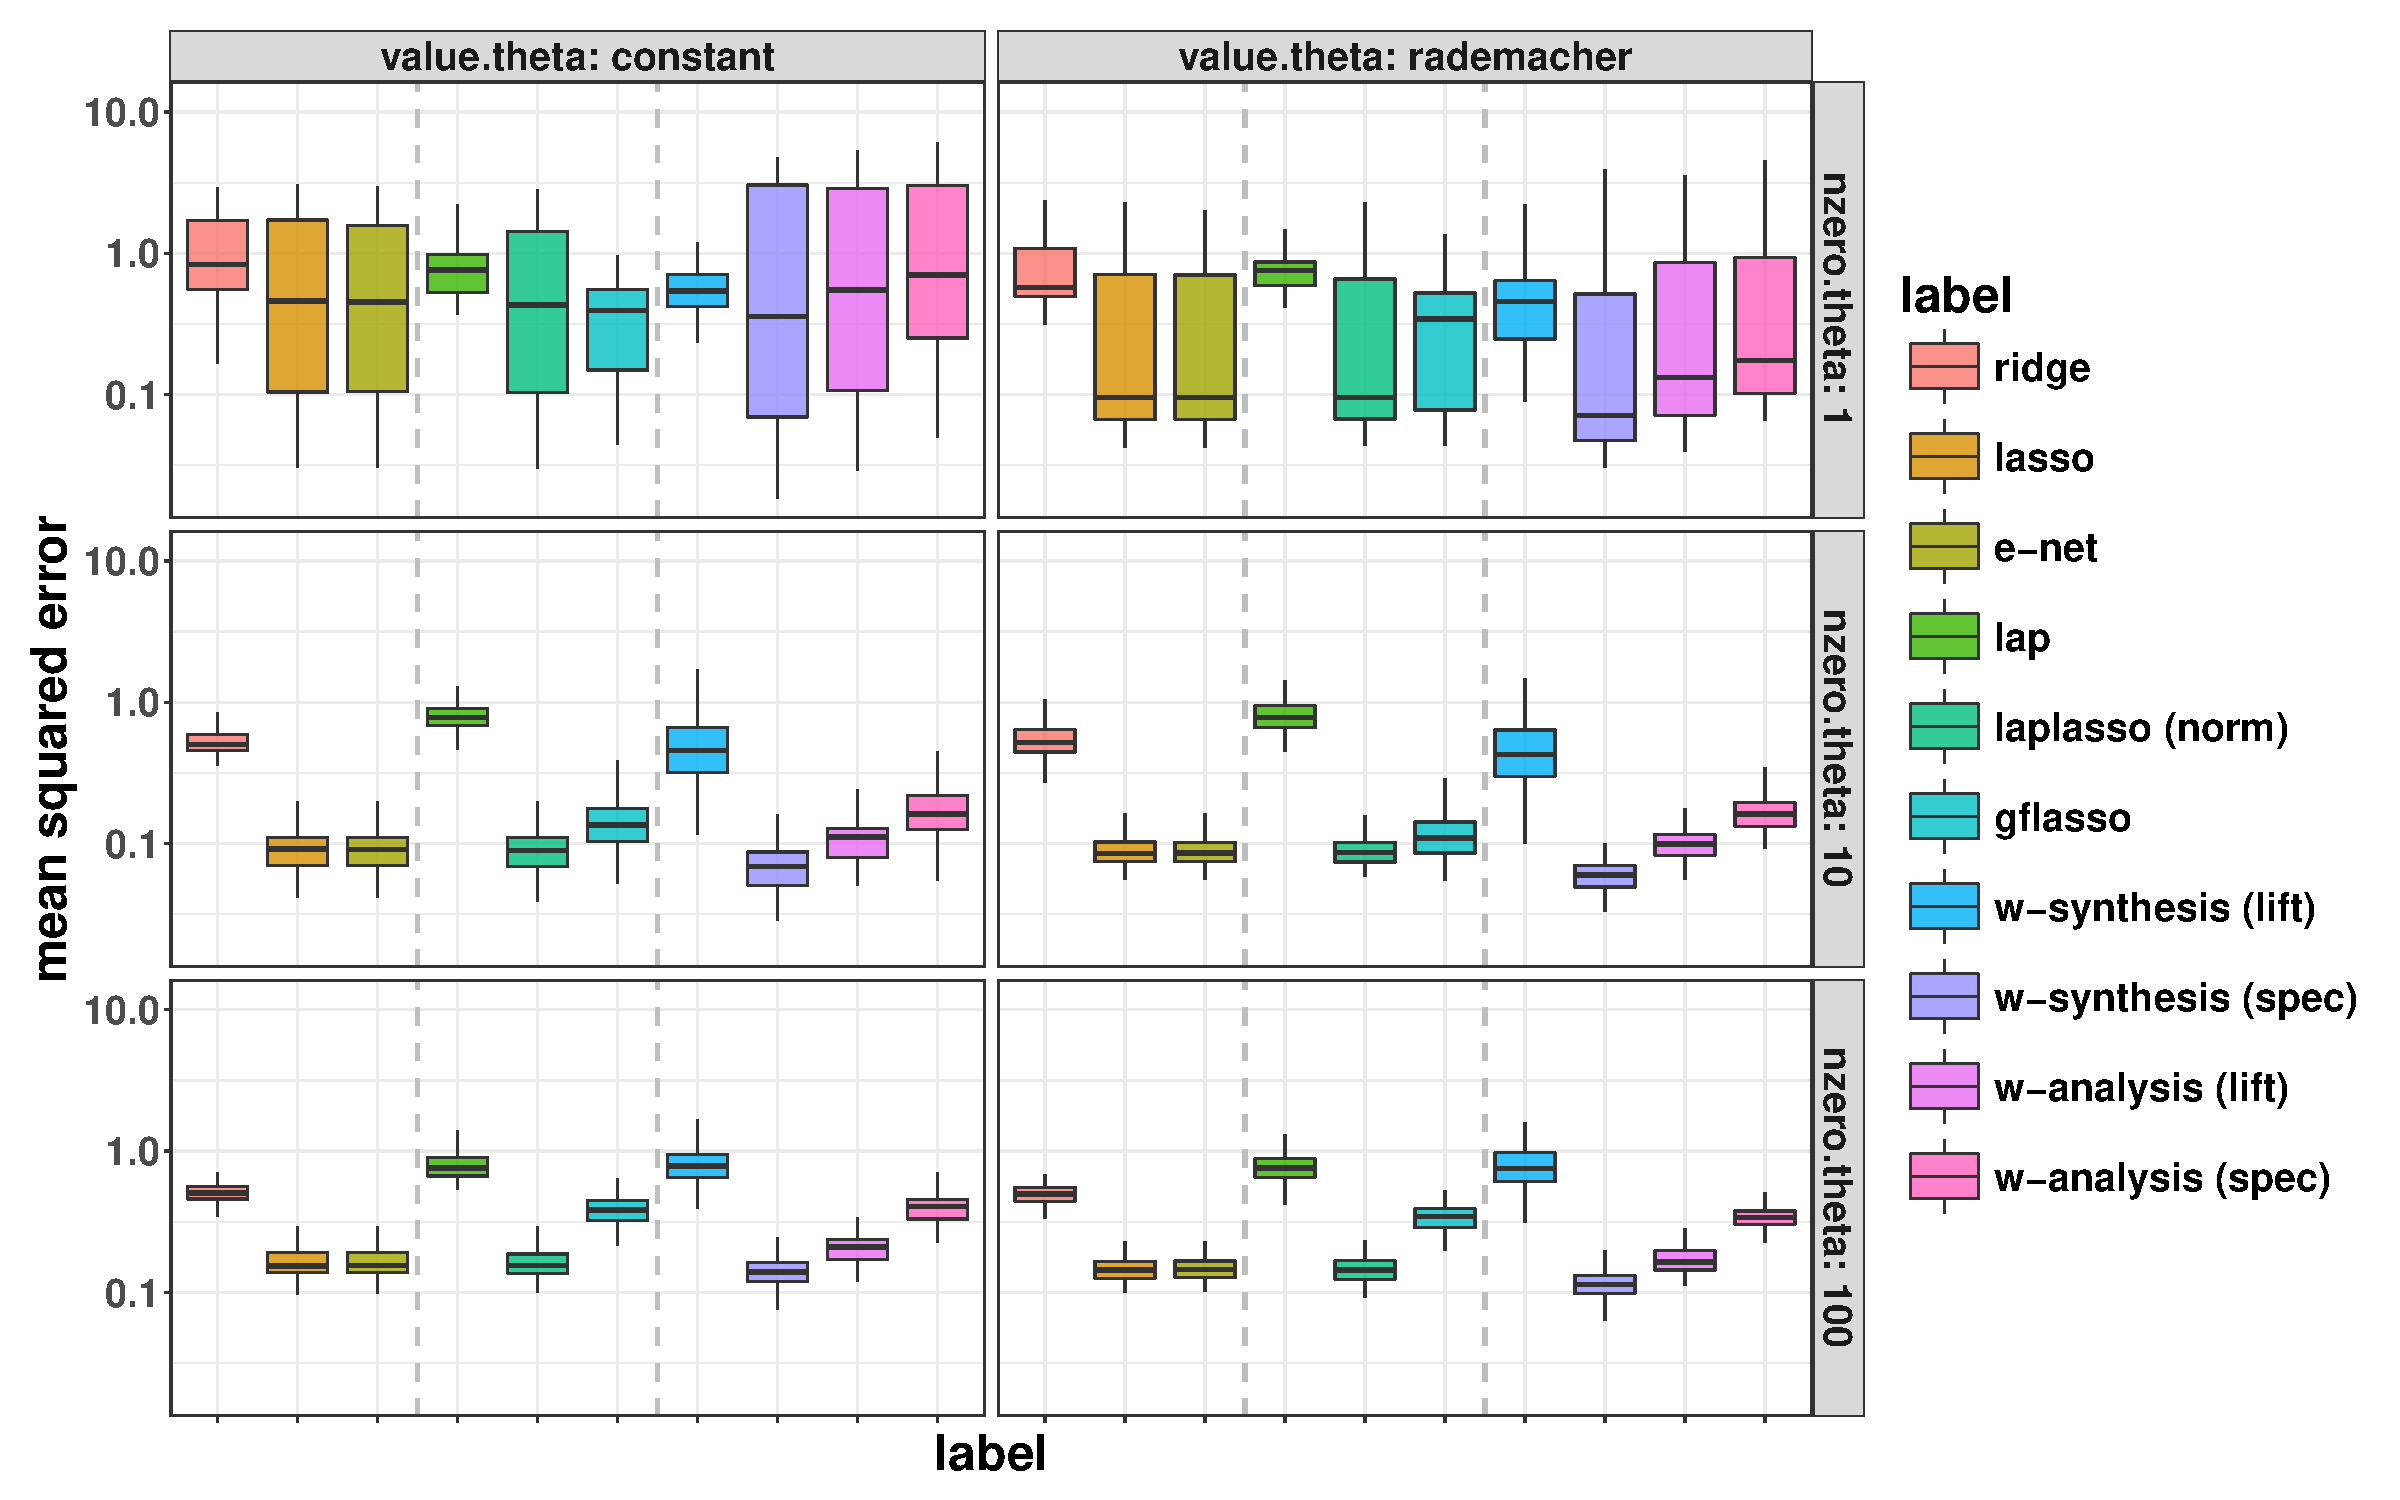
\includegraphics[width=0.9\textwidth]{ch-wavelet/plot-simulation}
	\caption{Boxplots on regression performance evaluated by prediction mean squared error over the $100$ training and test splits of the simulated data.}
	\label{fig3:simulation}
\end{figure}






On each simulated dataset, we performed $5$-fold cross-validation and evaluated the prediction mean squared error (PMSE) on each test fold, while the regularization parameters ($\lambda$ and $\nu$) were determined by nested cross-validation on each training fold. Results are shown in Figure \ref{fig3:simulation} where, under each combination of simulation set-up, boxplots present the PMSE over the $20 \times 5 = 100$ training and test splits of simulated data for a total of $10$ regularization methods including related variants. For all simulation set-ups, the wavelet-synthesis method with spectral graph wavelets denoted by ``\wsynspec{}'' is the consistent winner as expected, due to the fact that the simulated data are generated so that the informative features form locally connected subnetworks whose shapes and sizes are coherent with the spectral graph wavelets by design. The superiority is most striking when $\theta$ takes a reasonably intermediate number of non-zero coordinates, denoted by ``nzero.theta: 10'', and values that oscillate in sign, denoted by ``value.theta: rademacher''. Further, we observed that the same method with lifting-based graph wavelets instead of spectral graph wavelets, denoted by ``w-synthesis (lift)'', surprisingly exhibits the worst performance overall among all wavelet-based methods, which suggests that different approaches for constructing graph wavelets result in distinct characteristics and behaviors of underlying wavelets. However, the wavelet-analysis method is better suited with lifting-based graph wavelets than with spectral graph wavelets under our simulation set-ups, for which reasons remain unclear. Despite that the lasso and the elastic net are network-free methods, they still give competitive performance compared to the network-based Laplacian lasso or even outperform the network-based graph fused lasso in general in terms of PMSE. The two methods that do not allow for feature selection, namely the ridge and the Laplacian regularization, yield the worst prediction performance, due to the fact that the simulated data are generated by a sparse model involving only a few informative features.







\begin{figure}[!htbp]
	\centering
	\begin{subfigure}{0.9\textwidth}
		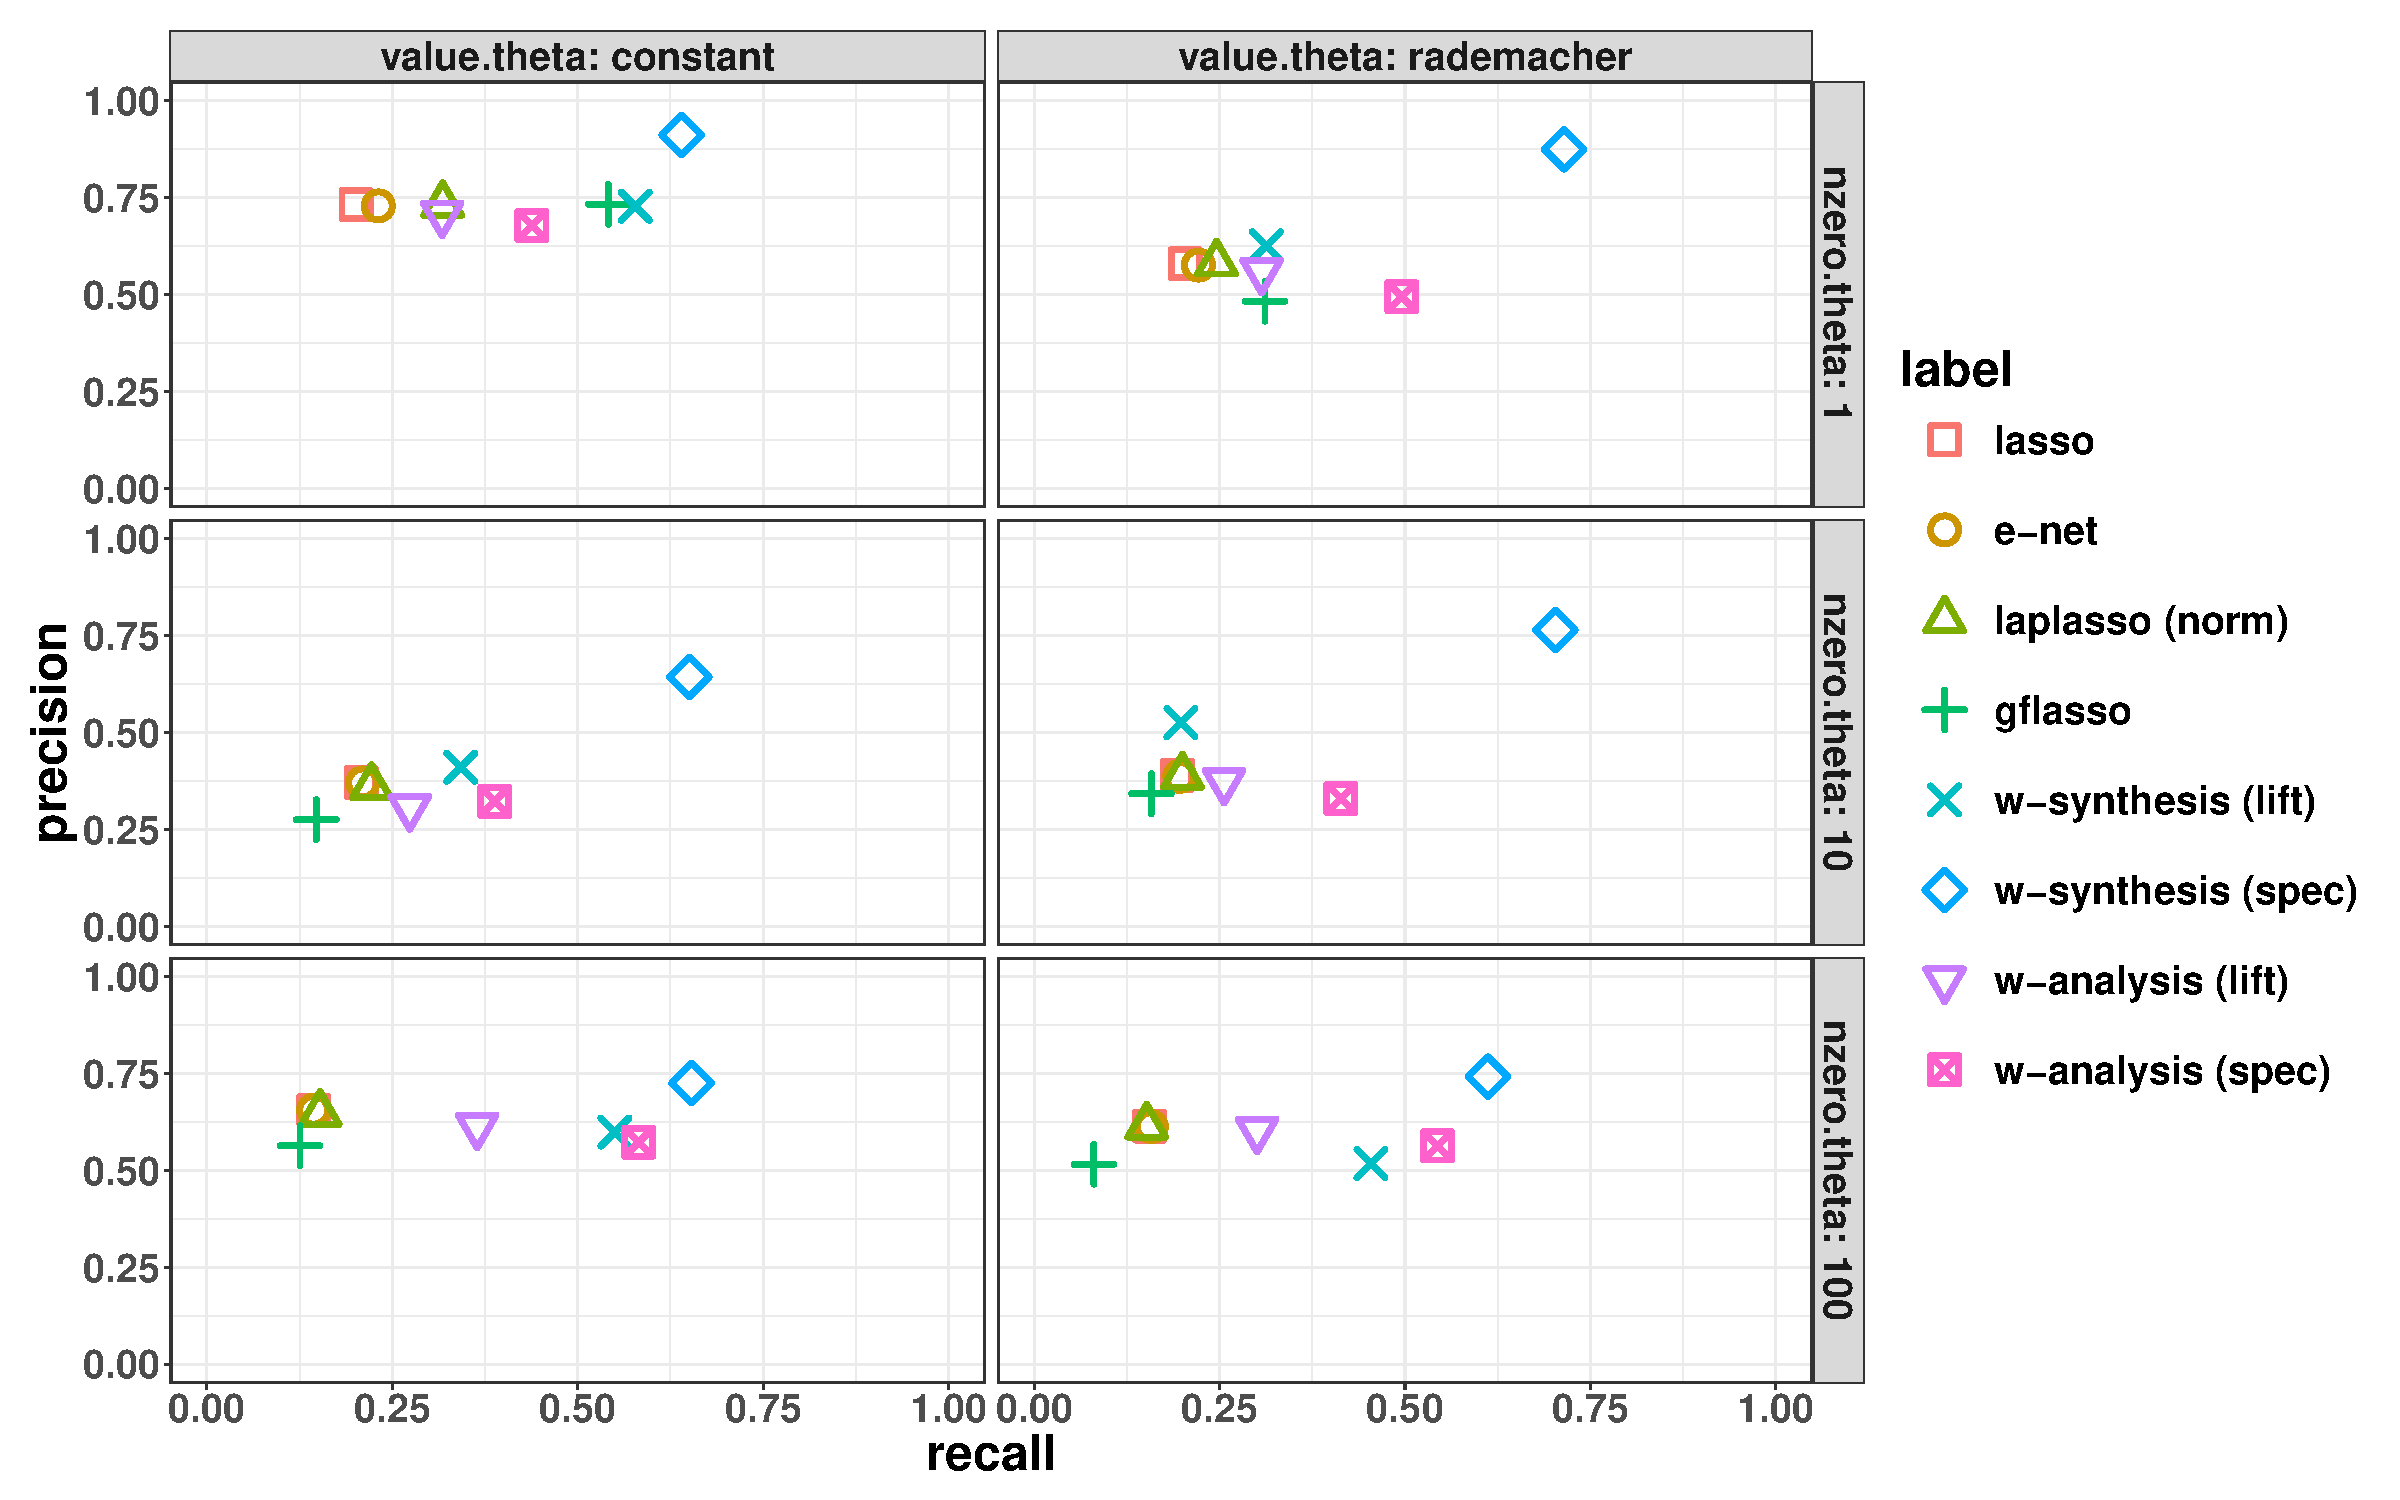
\includegraphics[width=\textwidth]{ch-wavelet/plot-support-beta}
		\caption{Support recovery of the coefficient vector $\beta$.}
		\label{fig3:support-beta}
	\end{subfigure}
	
	\begin{subfigure}{0.9\textwidth}
		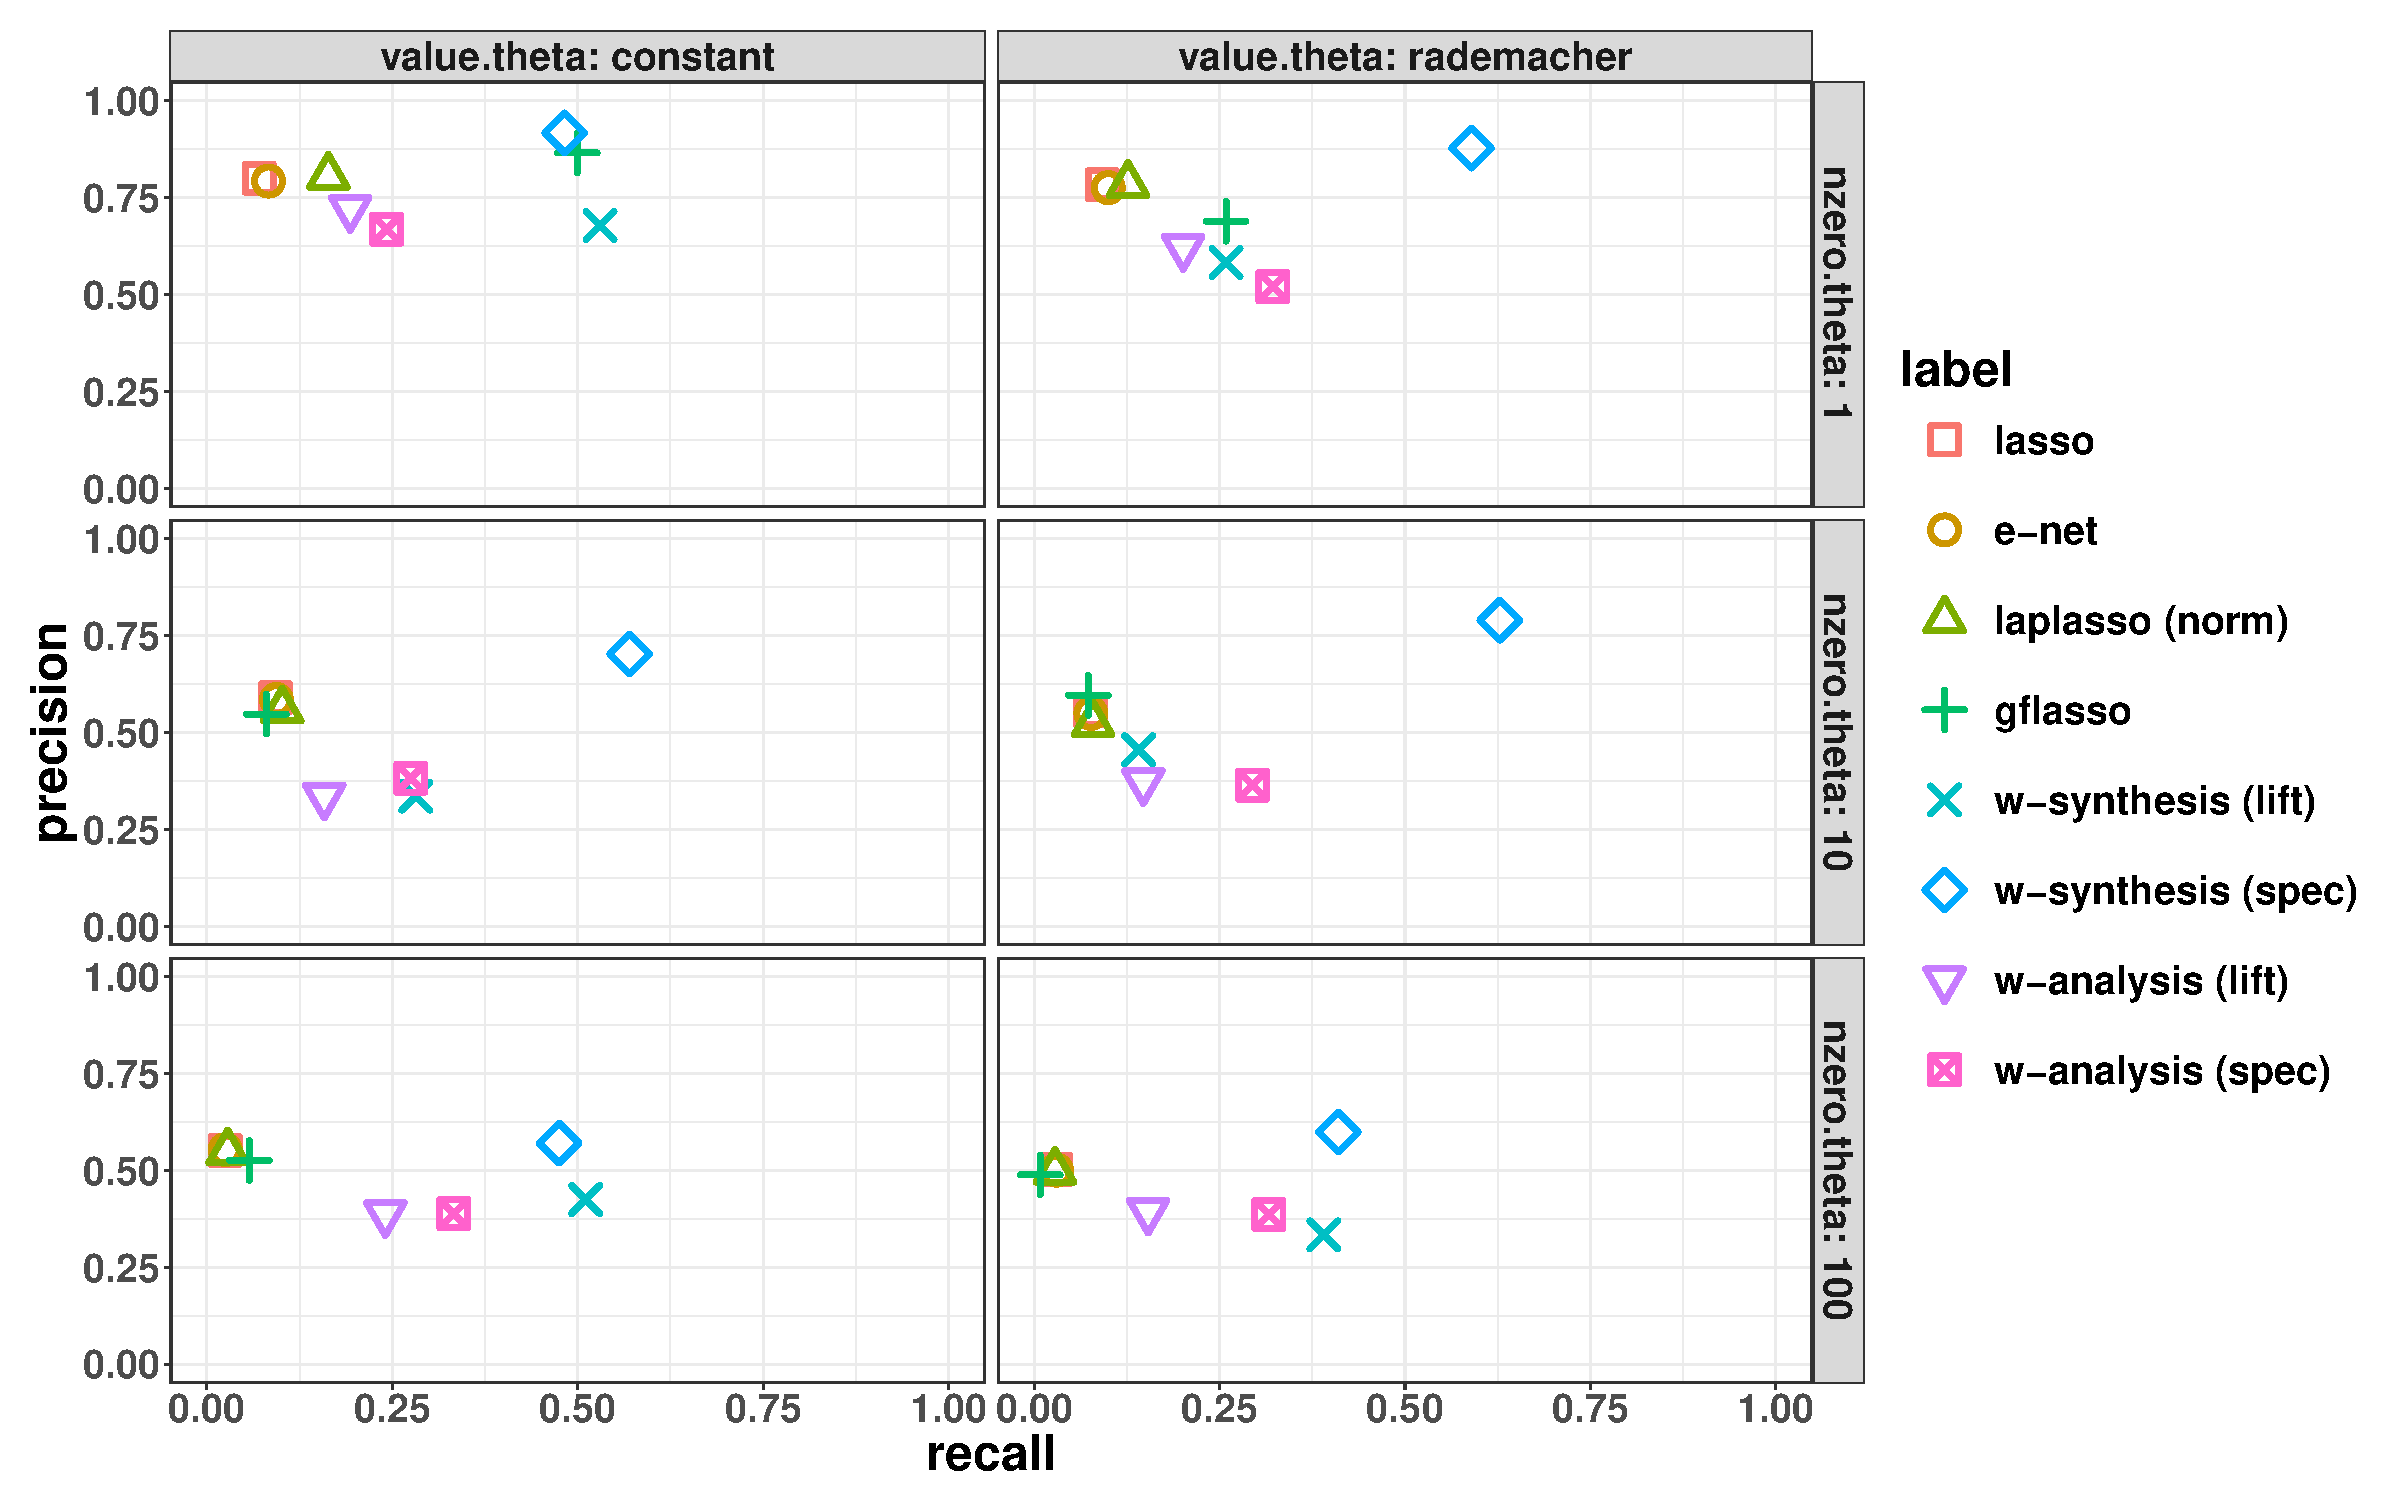
\includegraphics[width=\textwidth]{ch-wavelet/plot-support-edge}
		\caption{Support recovery of the connecting edges over the network.}
		\label{fig3:support-edge}
	\end{subfigure}
	\caption{Precision-recall plots on the recovery of simulated support of the coefficient vector $\beta$ and the connecting edges over the network.}
	\label{fig3:support}
\end{figure}







We further studied the sparsity-inducing methods which allow for feature selection regarding their ability to recover the informative features as well as the connecting edges over the network. Specifically, under a specific combination of simulation set-up, we applied each regularization method to each simulated dataset and obtained an estimate of $\beta$. We then compared the support as well as the connecting edges over the network underlying the estimated and true $\beta$ in terms of precision (the fraction of selected features that are truly informative) and recall (the fraction of truly informative features that are selected). In fact, as most values in $\beta$ are very small but not exactly zero in some cases, the ``non-zero'' support of $\beta$ is defined as the coordinates whose values are greater than one-hundredth of the largest value in $\beta$. For ease of visualization, we fit an ellipse over all the precision-recall points over the total of $20$ simulated datasets for each method, and the ellipse centers are shown in Figure \ref{fig3:support} for a total of $8$ methods including related variants. Again, the method denoted by ``\wsynspec{}'' is predominant as expected in terms of support recovery, most remarkably when $\theta$ takes a reasonably intermediate number of non-zero coordinates, denoted by ``nzero.theta: 10'', resulting in a modest number of connected subnetworks formed by the support of $\beta$. Compared to other methods, the wavelet-based methods generally tend to achieve competitive precision but much higher recall for the recovery of $\beta$ and the connecting edges over the network. Surprisingly, when the number of informative features becomes large and hence more connected over the network, the network-based Laplacian lasso and graph fused lasso does not distinguishingly outperform the network-free lasso and elastic net in terms of feature selection or even edge identification.









\subsection{Breast Cancer Survival Analysis}
\label{sec3:breastcancer}


For \textit{in vivo} experiments, we performed survival analysis for breast cancer using the METABRIC data guided by the HPRD PPI network. In fact, for each breast tumor sample, the METABRIC dataset additionally provides clinical information on the overall survival time of the underlying patient, that is either the exact number of days dating from initial consultation until the patient passed away or the number of days until the patient is last seen alive. This clinical information was converted to right-censored survival data and we performed survival risk prediction for breast cancer.








\begin{figure}[!htbp]
\centering
	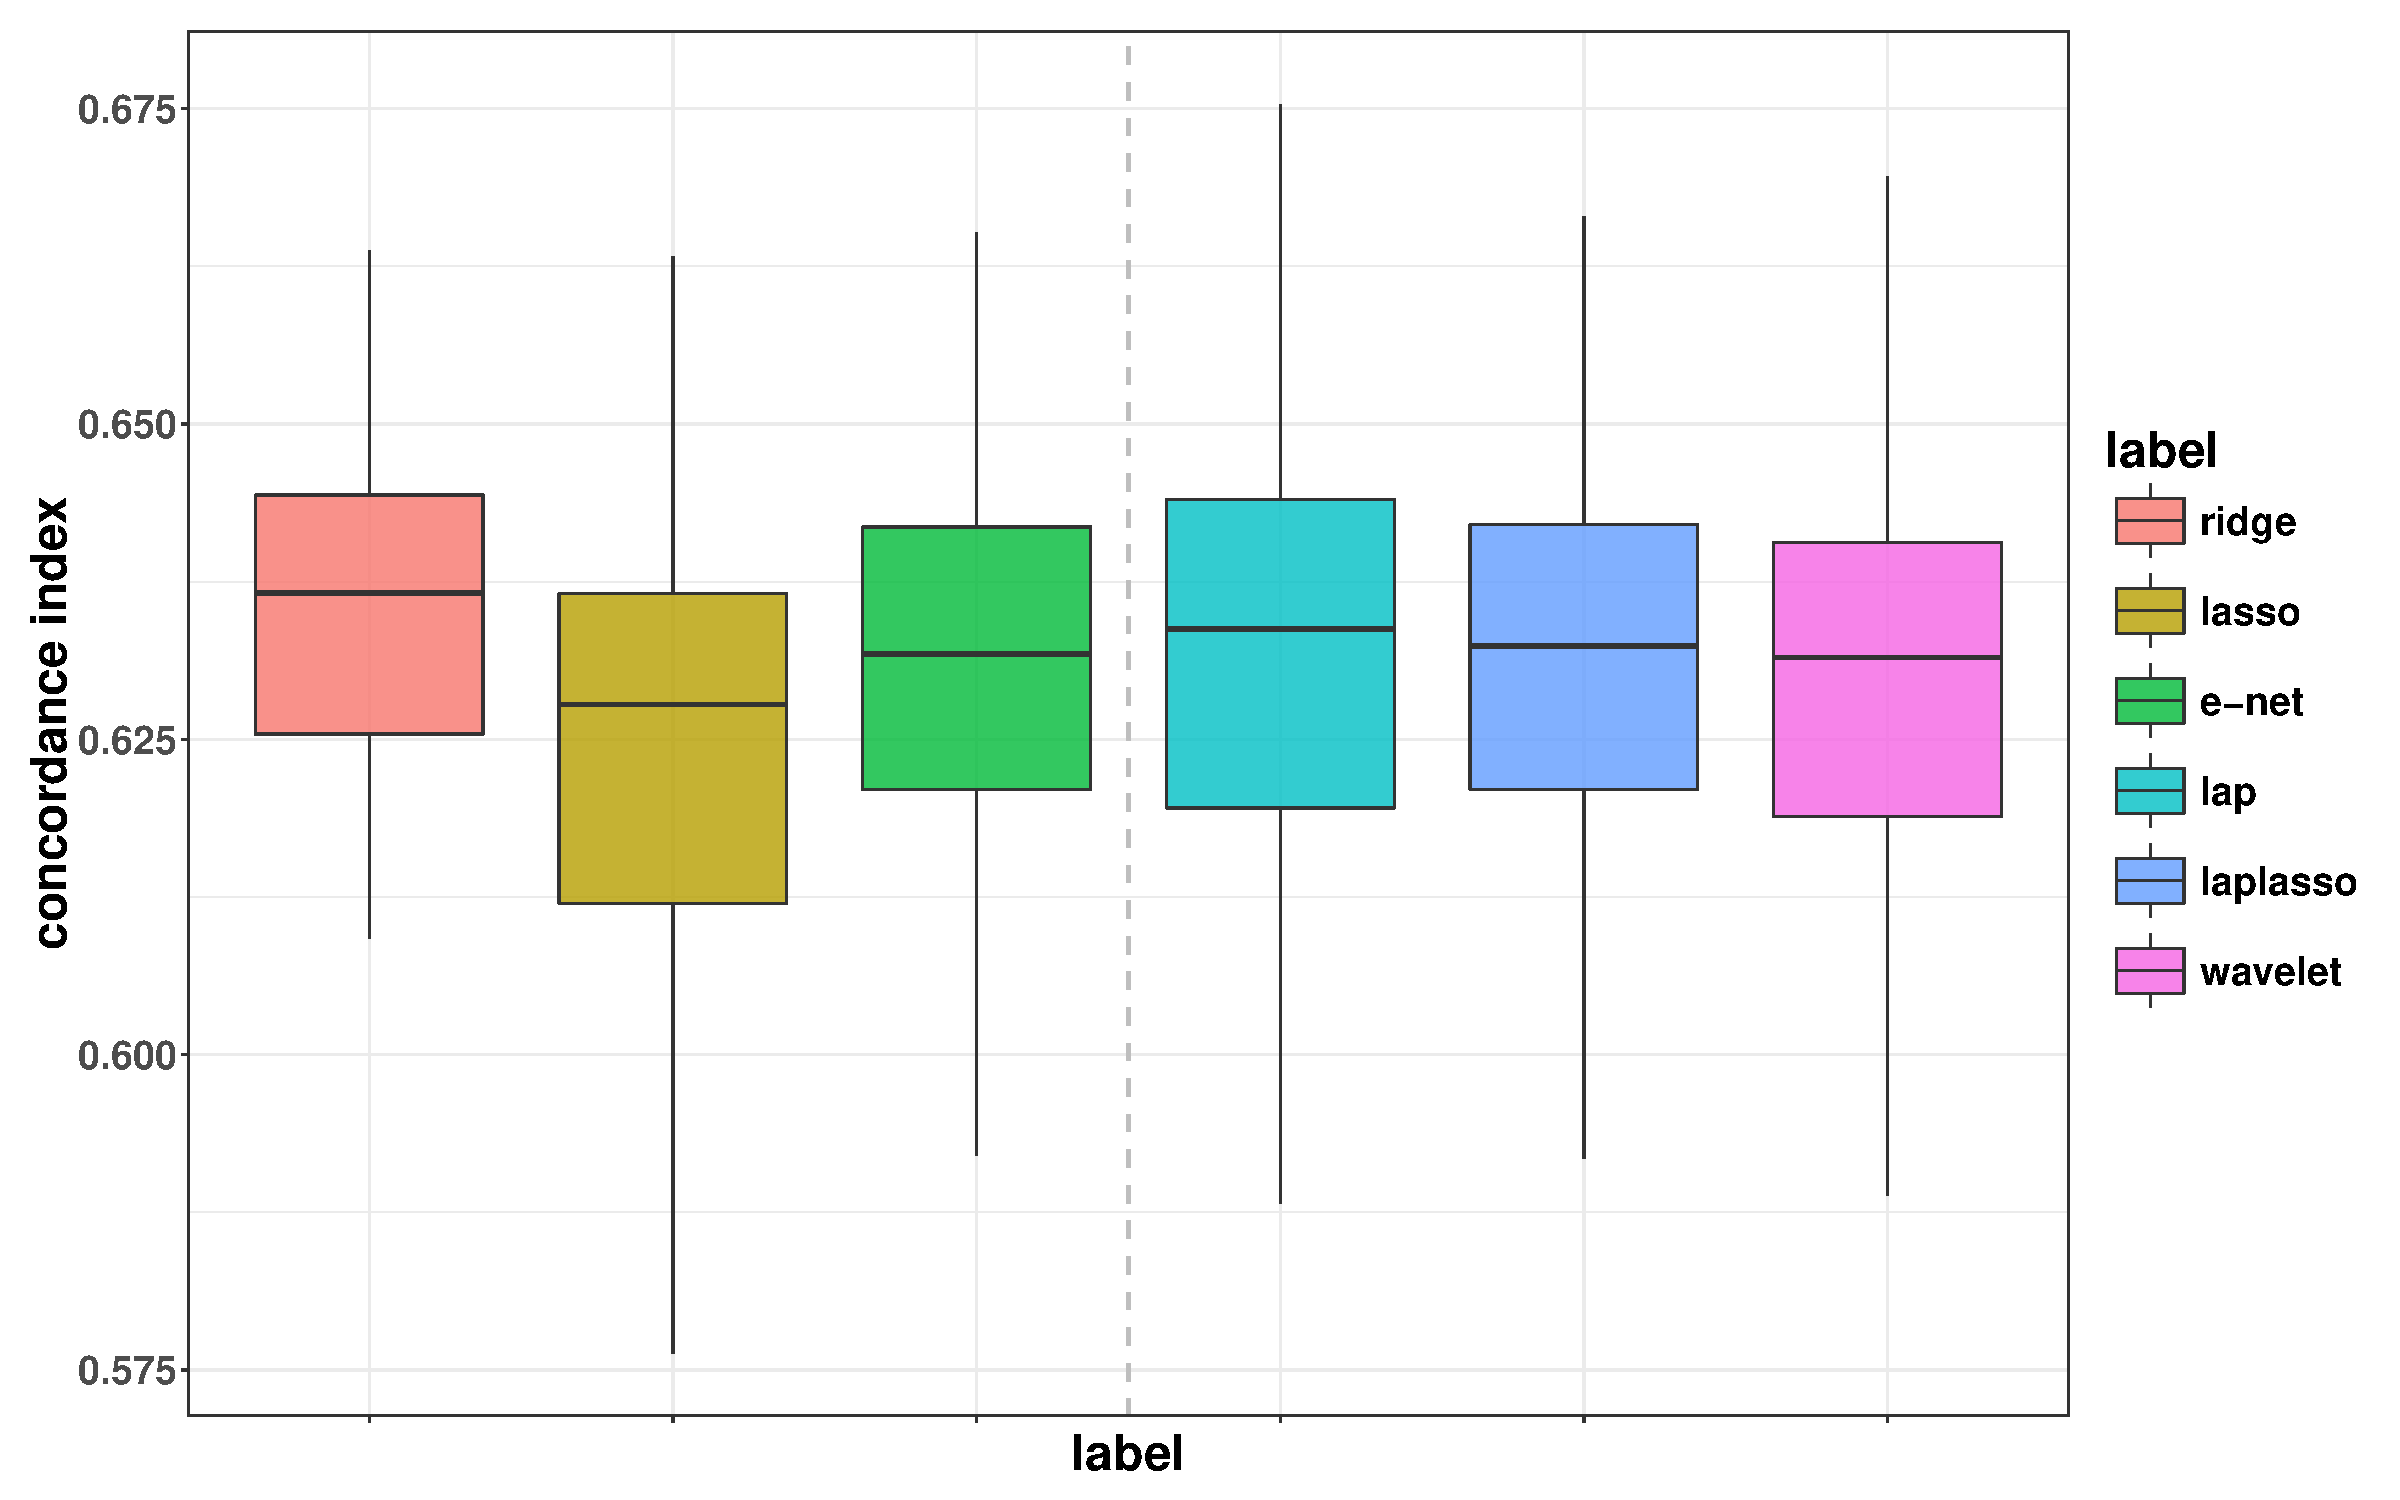
\includegraphics[width=0.9\textwidth]{ch-wavelet/plot-prediction}
	\caption{Boxplots on survival risk prediction performance evaluated by concordance index scores over 5-fold cross-validation repeated 10 times of the METABRIC data.}
	\label{fig3:prediction}
\end{figure}



\begin{table}[!htbp]
\centering
\caption{Mean concordance index (CI) scores ($\pm$ standard deviation) of survival risk prediction over 5-fold cross-validation repeated 10 times of the METABRIC data. Methods are ordered by decreasing mean CI scores.}
\small
	\begin{tabular}{c|c|c|c}
	\hline
	Label & Mean CI scores ($\pm$ SD) & Network-based & Feature selection \\\hline
	ridge (org)	&	$0.637 \, (\pm 0.0178$)	&	& \\
	ridge	&	$0.636 \, (\pm 0.018$)	&	& \\
	e-net (org)	&	$0.6345 \, (\pm 0.0185$)	&	& $\checkmark$ \\
	lap (norm)	&	$0.633 \, (\pm 0.0196$)	& $\checkmark$	& \\
	lap	&	$0.632 \, (\pm 0.0193$)	& $\checkmark$	& \\
	laplasso (norm)	&	$0.6312 \, (\pm 0.0185$)	& $\checkmark$	& $\checkmark$ \\
	e-net	&	$0.6304 \, (\pm 0.0183$)	&	& $\checkmark$ \\
	\wanaspec	&	$0.6295 \, (\pm 0.0198)$	& $\checkmark$	& $\checkmark$ \\
	\wsynspecnorm	&	$0.6264 \, (\pm 0.018)$	& $\checkmark$	& $\checkmark$ \\
	lasso	&	$0.626 \, (\pm 0.0177)$	&	& $\checkmark$ \\
	lasso (org)	&	$0.6257 \, (\pm 0.0172)$	&	& $\checkmark$ \\
	\wanaspecnorm	&	$0.6216 \, (\pm 0.0228)$	& $\checkmark$	& $\checkmark$ \\
	w-analysis (lift)	&	$0.6163 \, (\pm 0.0182)$	& $\checkmark$	& $\checkmark$ \\
	\wsynspec	&	$0.6157 \, (\pm 0.0184)$	& $\checkmark$	& $\checkmark$ \\
	w-synthesis (lift)	&	$0.5587 \, (\pm 0.0232)$	& $\checkmark$	& $\checkmark$ \\
	\hline
	\end{tabular}
\label{tab3:prediction}
\end{table}







The first objective of the \textit{in vivo} investigation is to compare the survival risk prediction performance of different regularization methods. To this end, we performed $5$-fold cross-validation repeated $10$ times on the full METABRIC dataset and evaluated the concordance index (CI) scores on each test fold, while the regularization parameters ($\lambda$ and $\nu$) were determined by nested cross-validation on each training fold. Note that CI is a measure of rank-based consistency between the predicted survival risk and observed survival time for a cohort of patients, in the sense that it is an estimate of the probability that, given two randomly drawn patients, the patient who survives longer is predicted with a lower risk. Results are shown in Figure \ref{fig3:prediction} with boxplots over the $10 \times 5 = 50$ splits of training and test data and in Table \ref{tab3:prediction} with mean CI scores ($\pm$ standard deviation) for a total of $15$ regularization methods including related variants. The ridge is the best-performing model in terms of mean CI scores but it does not allow for feature selection, and among methods that enable feature selection, the elastic net is the best-performing one. Notably, both methods are regardless of the prior knowledge encoded in the network. Among network-based methods that enable feature selection, the best-performing one is the Laplacian lasso, followed by the wavelet-analysis method with spectral graph dual wavelets. We observed that the wavelet-based methods provide relatively less accurate survival risk prediction in terms of CI scores compared to other methods. We performed two-sided t-tests to statistically quantify the difference of the cross-validation CI scores between each pair of methods. FDR-adjusted p-values suggest that, at the significance level $0.05$, there is no significant decrease in the prediction performance for the best-performing wavelet-based method, namely the method denoted by ``\wanaspec{}'', compared to any of the methods tested. Notably, network-free methods using the entire list of genes available from the METABRIC data does not significantly improve the survival risk prediction performance, compared to those using the subset of genes only found on the HPRD PPI network. This justifies that the loss is not significant when our analysis is restrained to the subset of genes found on the network. For detailed results regarding the statistical tests, we refer to the online supplements. Another interesting observation regarding wavelet-based methods is that, as the spectral graph wavelets are constructed using graph Laplacian that appear in either normalized or non-normalized version, the wavelet-analysis method is better suited with the non-normalized version while the wavelet-synthesis method is better suited with the normalized version, for which reasons remain unclear.










The focus of \textit{in vivo} experiments in this study is to select genes that are related to breast cancer survival, and in particular we favor methods that result in a list of selected genes that tend to form gene modules on the HPRD PPI network potentially by making use of their biological interaction known \textit{a priori}. To this end, we then compared the goodness of gene selection of different methods from several aspects, namely stability, connectivity and interpretability. Note that only those $9$ methods including related variants that enable feature selection are discussed for the remainder of this section.









\begin{figure}[!htbp]
\centering
	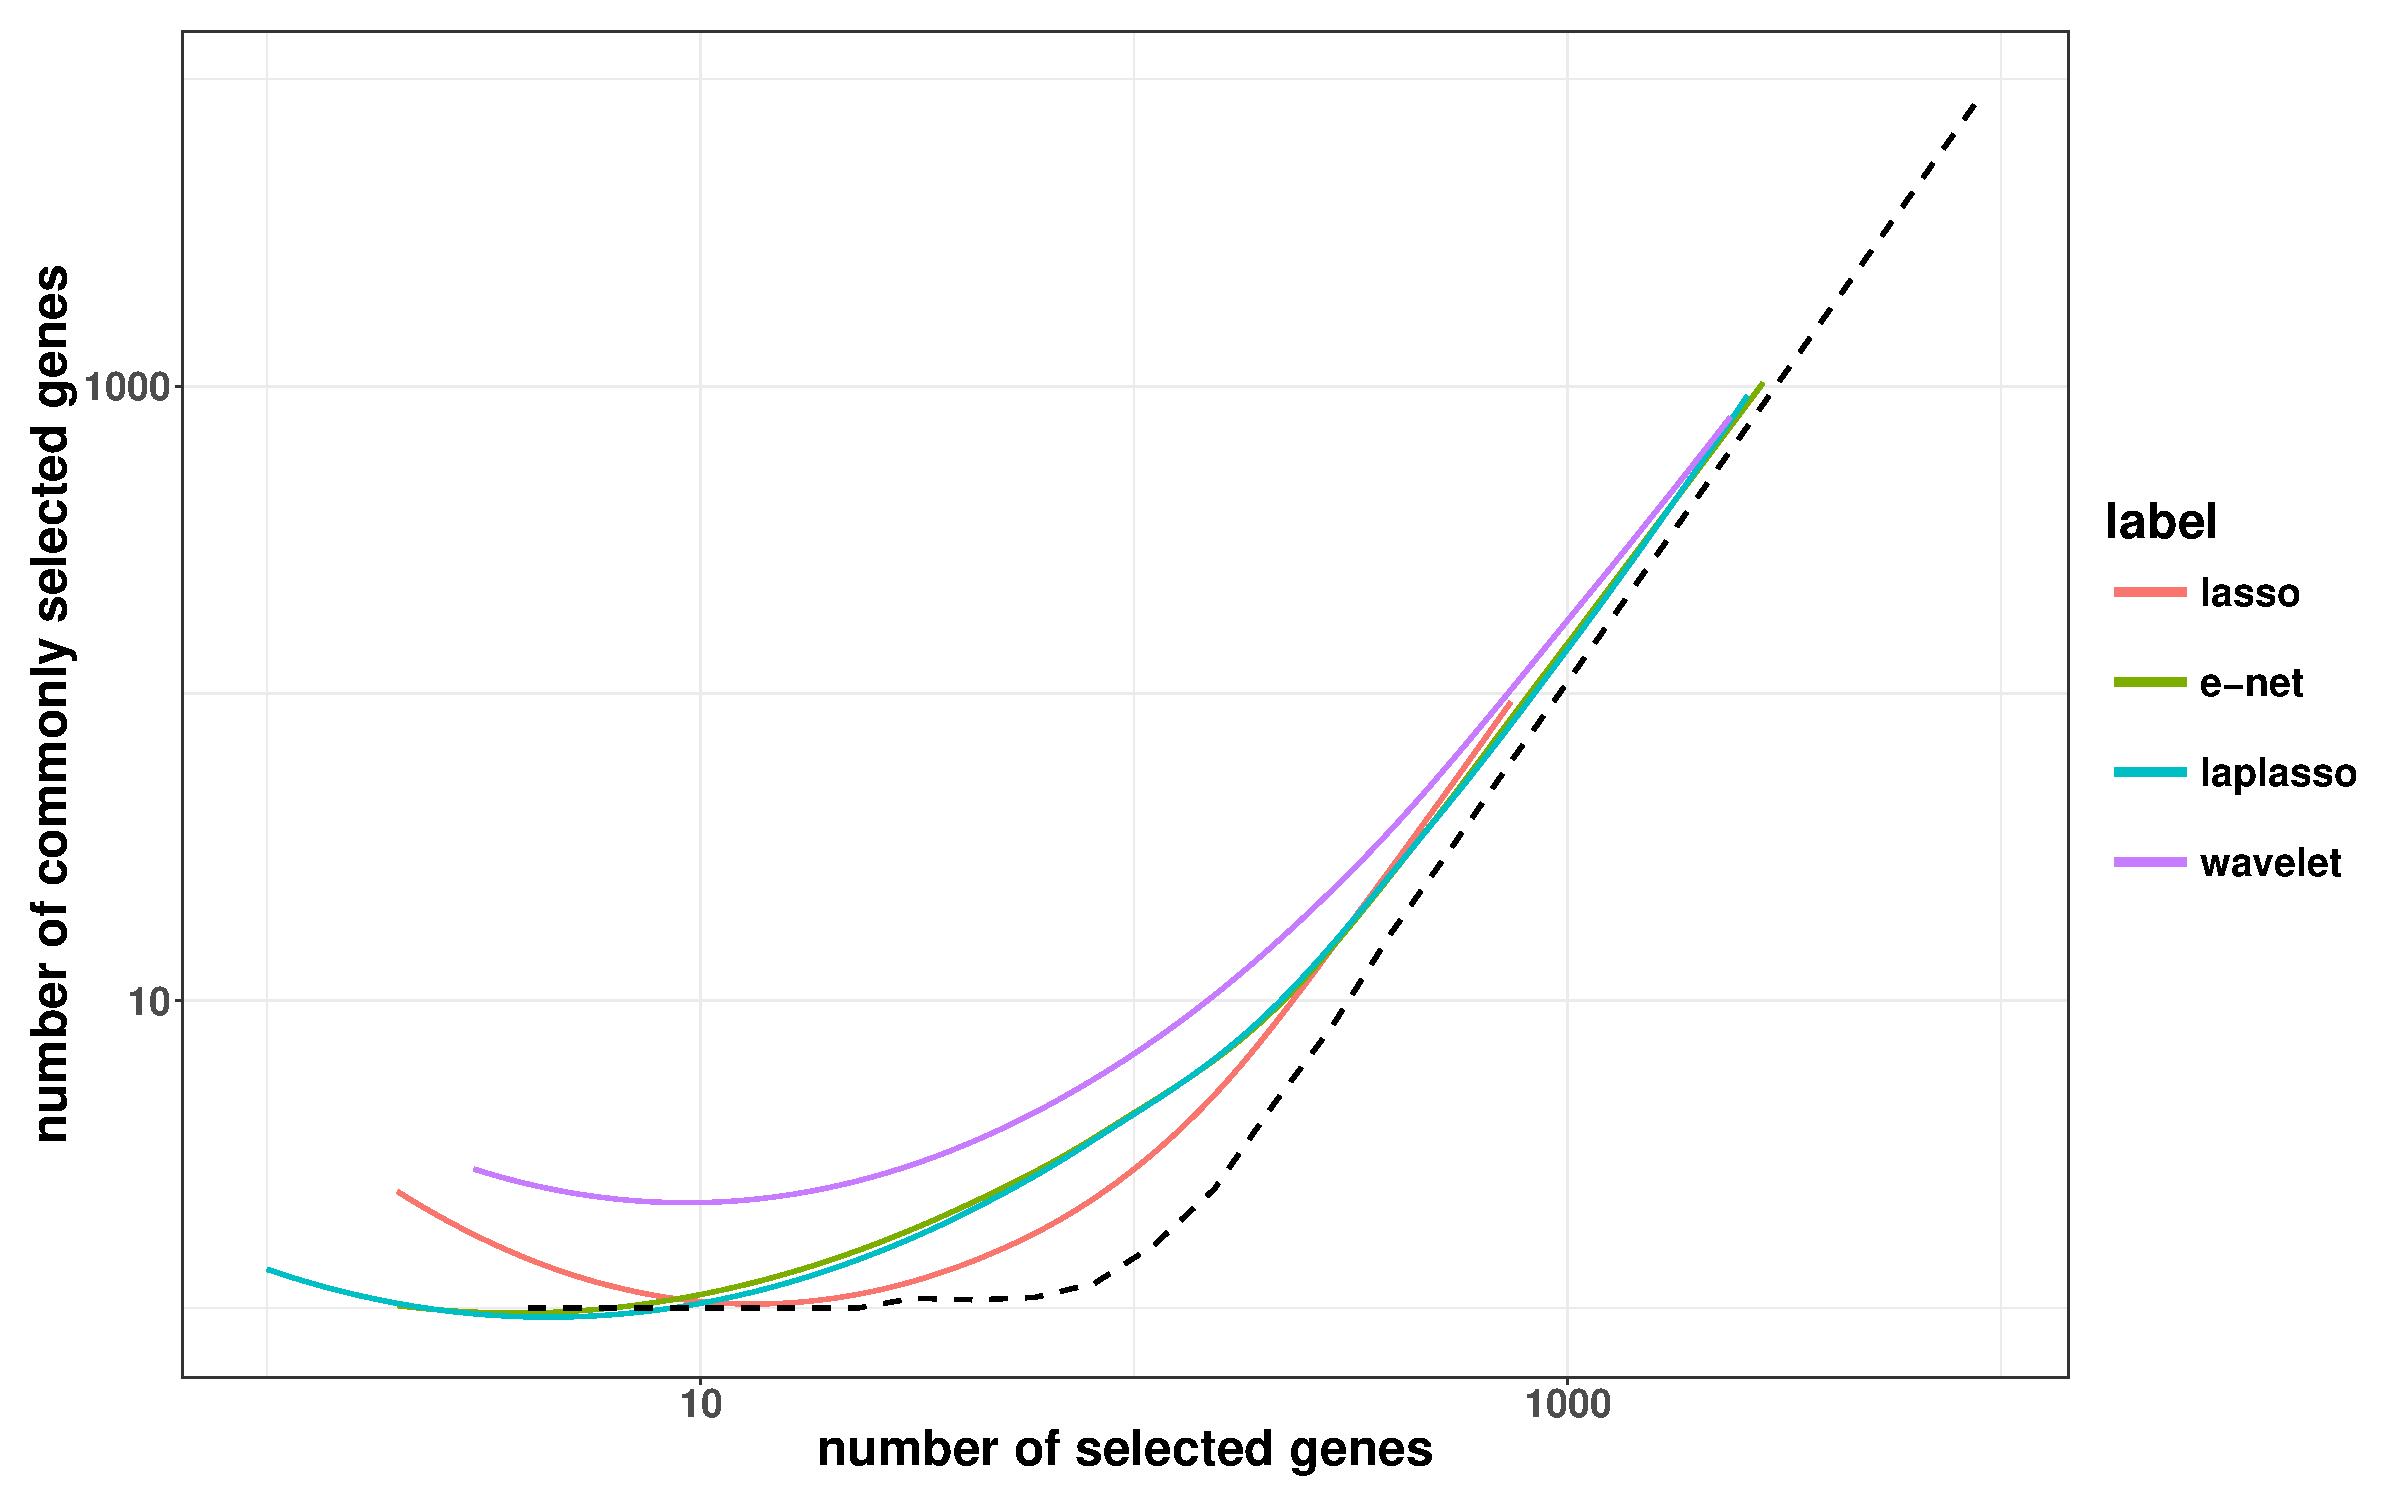
\includegraphics[width=0.9\textwidth]{ch-wavelet/plot-stability}
	\caption{Stability performance of gene selection related to breast cancer survival, estimated over $100$ random experiments. The black dotted curve denotes random selection.}
	\label{fig3:stability}
\end{figure}




Stability is an important concept that advocates reproducibility of selecting the significant features across independent studies. In order to compare stability of feature selection by different methods, we randomly split the full METABRIC dataset evenly into two halves and obtained a pair of models independently trained on the two disjoint subsets with the same method. Then constraining on each fixed number of genes selected, we computed the number of commonly selected genes between the two independent models as a score indicating stability. We repeatedly split the data $100$ times to address the randomness in splitting the data. For ease of visualization, we applied locally weighted scatterplot smoothing (LOESS) \cite{Cleveland1979Robust} to all the stability scores for each method and thus obtained a curve of stability scores along the solution path. Results are shown in Figure \ref{fig3:stability}. We observed that the number of commonly selected genes between pairs of independent models tends to become larger as the number of selected genes increases. As we are most interested in selecting typically a few hundreds of genes that could interestingly form subnetworks of modest sizes, the wavelet-based method denoted by ``\wanaspecnorm{}'' distinguishingly won in terms of stability at the scale of $10^2$ genes selected, followed by two other wavelet-based methods denoted by ``\wanaspec{}'' and ``\wsynspec{}''. Recall that the method denoted by ``\wanaspec{}'' is the best-performing method in terms of CI scores for survival risk prediction. Last but not least, the network-free methods, namely the lasso and elastic net, and network-based Laplacian lasso provide feature selection procedures that are overall less stable. Further, as negative-control experiment, we randomly selected twice the same number of genes along the solution path and counted the number of commonly selected genes. At each fixed number of genes selected, the number of commonly selected genes is averaged over $100$ repeats to address the randomness. A stability curve for random selection is shown by the black dotted curve in the figure. Note that all methods tested in this study outperform the random selection in terms of stability, especially strikingly at the scale of $10^2$ genes selected.











\begin{figure}[!htbp]
\centering
	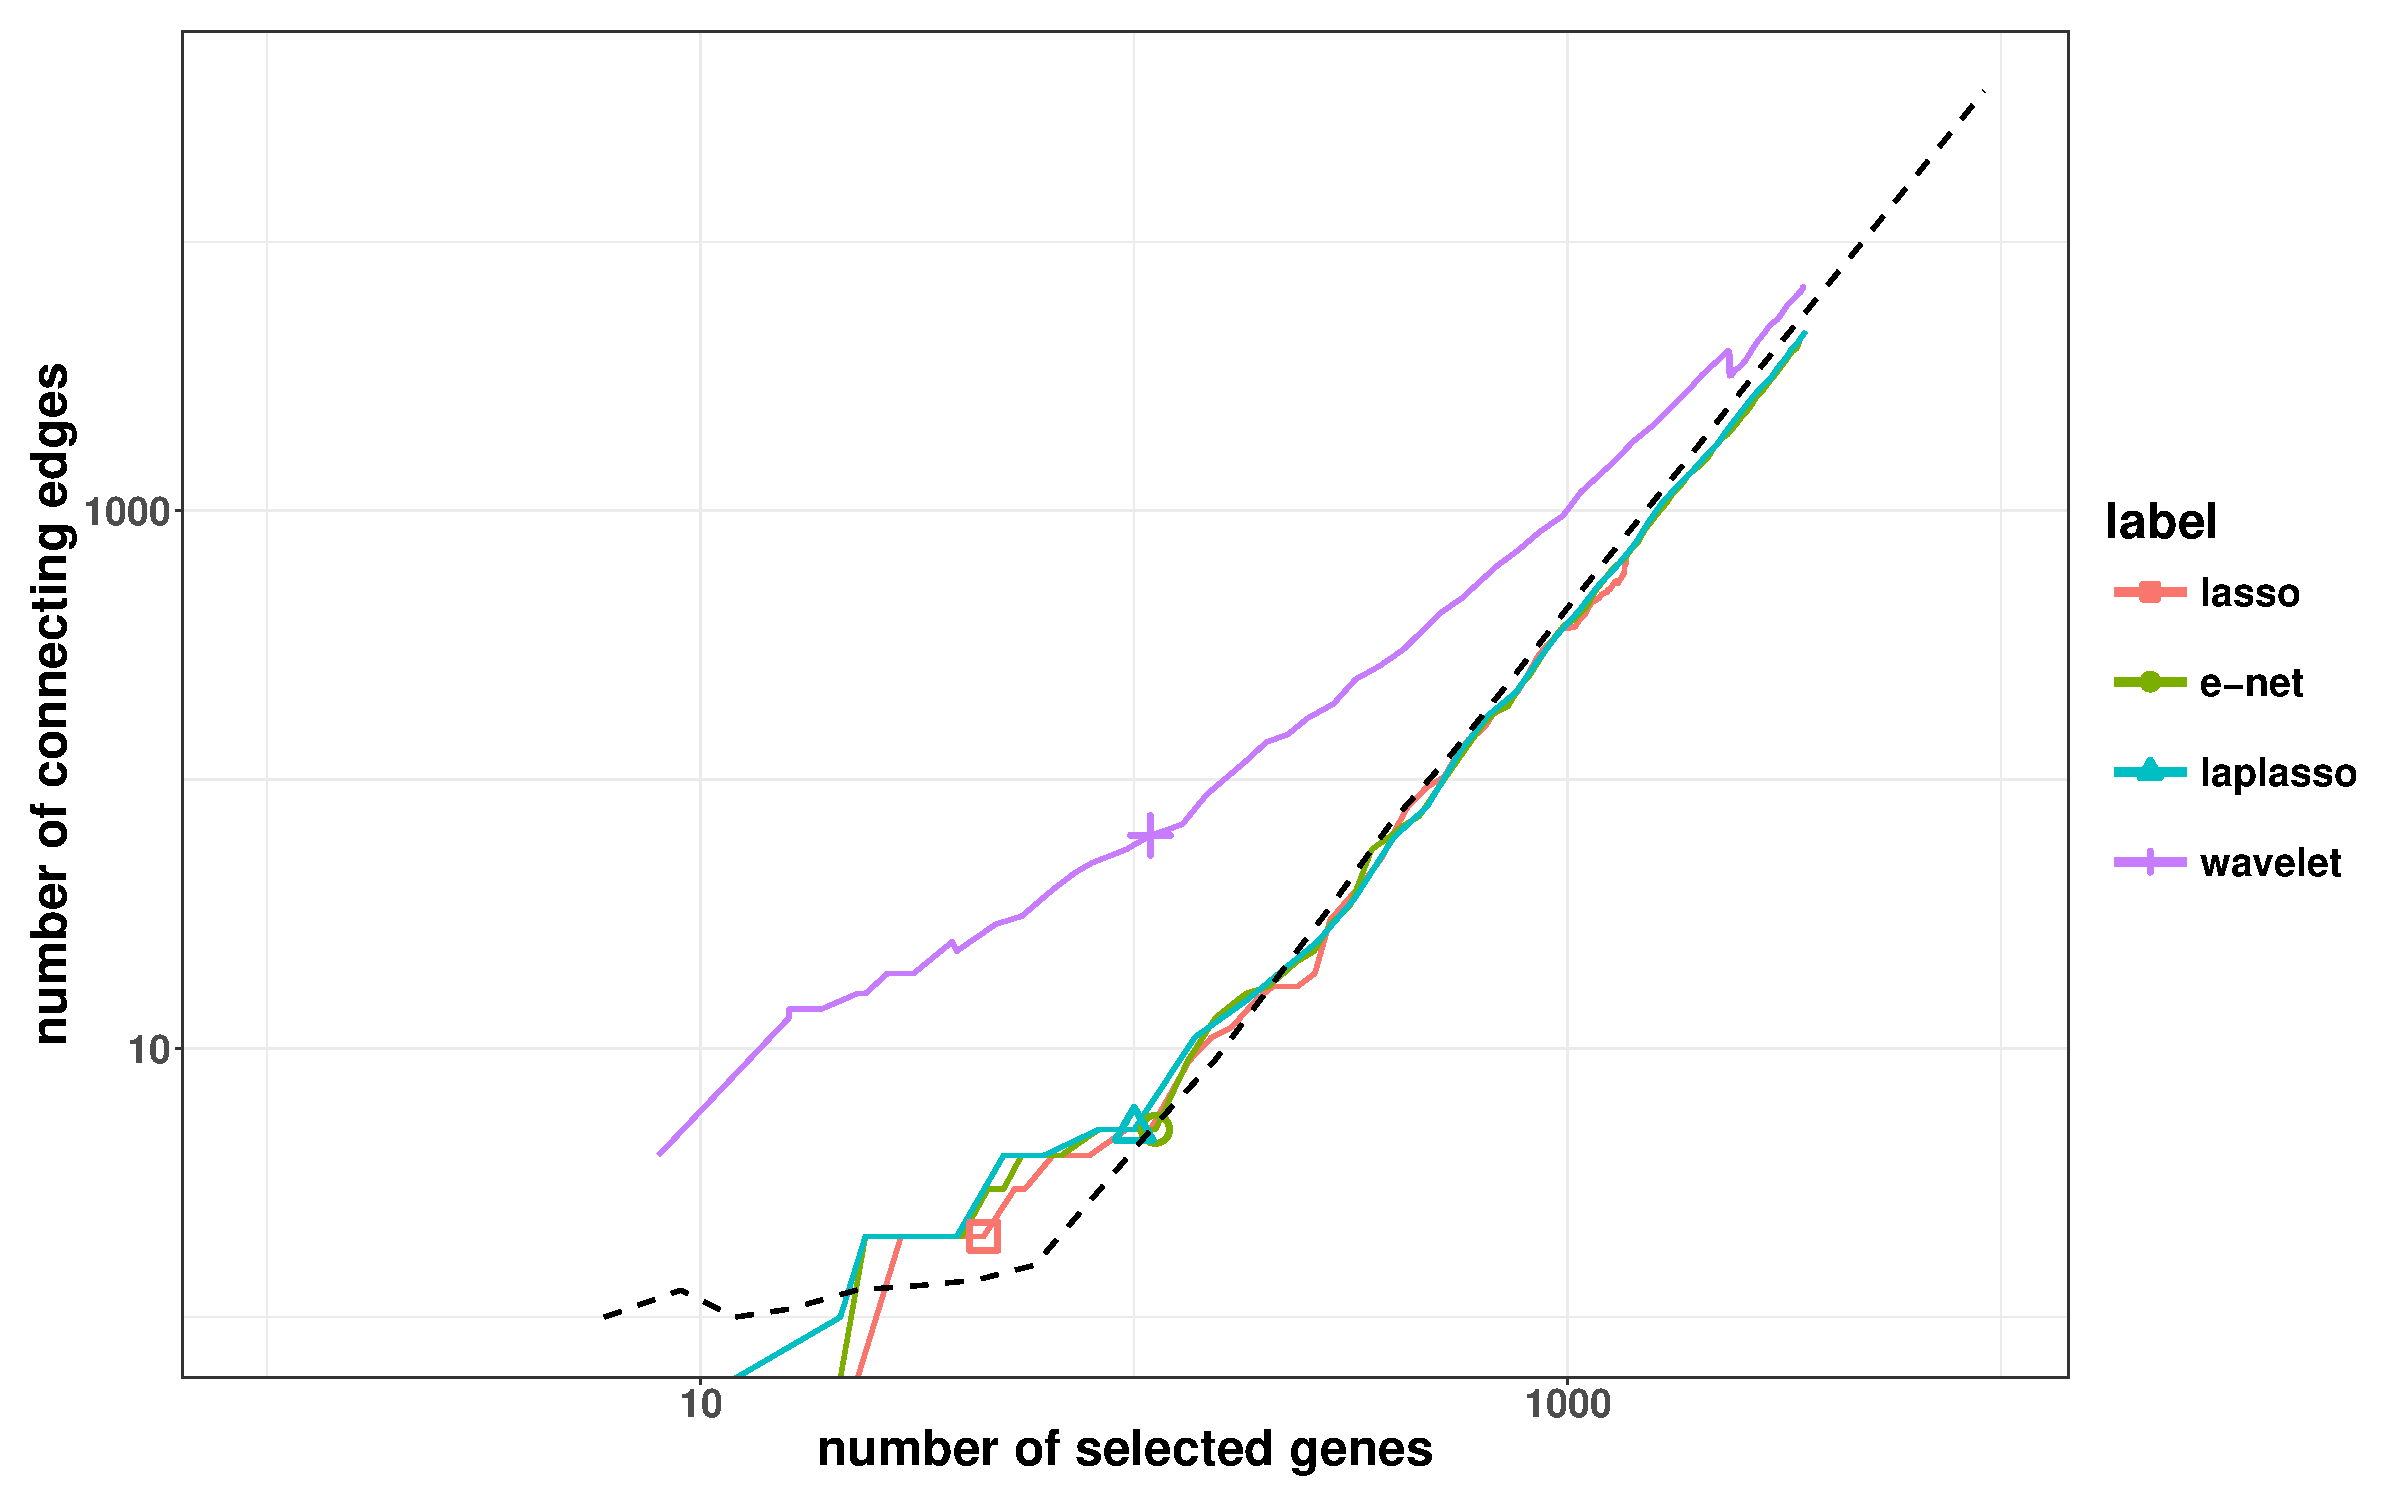
\includegraphics[width=0.9\textwidth]{ch-wavelet/plot-connectivity}
	\caption{Connectivity performance of gene selection related to breast cancer survival, where special marks correspond to the number tuned by cross-validation. The black dotted curve denotes random selection.}
	\label{fig3:connectivity}
\end{figure}







Recall from the introduction that the motivation of this study is to encourage selected features to be connected given a network, and for that purpose, we would like to quantitatively compare feature selection in terms of connectivity over the given network. A model is trained by applying each method to the full METABRIC dataset and, constraining on each fixed number of genes selected, a connectivity score is defined as the number of connecting edges between the selected genes. Thus for each method we obtained a curve of connectivity scores along the solution path. Results are shown in Figure \ref{fig3:connectivity}, where special marks indicate the number of genes and connecting edges that was determined by tuning the regularization parameter $\lambda$ by cross-validation. We observed that the wavelet-based methods remarkably outperform other methods in terms of connectivity in general. In particular, the method denoted by ``\wanaspecnorm{}'' that has stood out in terms of stability remains to be one of the top-performing methods in terms of connectivity, whereas it selected a relatively large number of genes by cross-validation. It is worth special mention that the method denoted by ``\wanaspec{}'' selected around $10^2$ genes by cross-validation that attain a reasonably good number of connecting edges, and it has been one of the top-performing methods in terms of stability in feature selection when this number of genes is selected, and it also remains competitive to all other methods in terms of CI scores for survival risk prediction. A side note on the strange performance of the method denoted by ``w-synthesis (lift)'' is that this method output an estimate of $\beta$ that is constant\footnote{Due to numerical instability in computation, there may exist infinitesimal variations in the values of estimated $\beta$ output by the method.} when fitted to the full METABRIC dataset particularly, and consequently the full list of genes were considered as selected. Further, as negative-control experiment, we randomly selected a certain number of genes regardless of a network, and counted the number of connecting edges over the given network. At each fixed number of genes selected, the number of connecting edges is averaged over $100$ repeats to address the randomness. A connectivity curve for random selection is shown by the black dotted curve in the figure. Note that the network-free methods, namely the lasso and the elastic net, and network-based Laplacian lasso do not seem to significantly outperform the random selection in terms of connectivity.







\begin{figure}[!htbp]
	\centering
	\begin{subfigure}{0.9\textwidth}
		\centering
		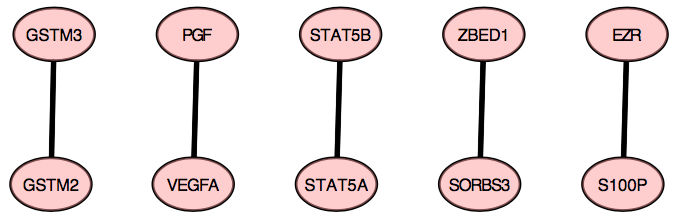
\includegraphics[width=0.5\textwidth]{ch-wavelet/subnetworks_e-net}
		\caption{Gene subnetworks identified by the elastic net ($10$ genes connected out of $112$ selected) or the Laplacian lasso ($10$ genes connected out of $100$ selected).}
		\label{fig3:enet}
	\end{subfigure}
	
	\begin{subfigure}{0.9\textwidth}
		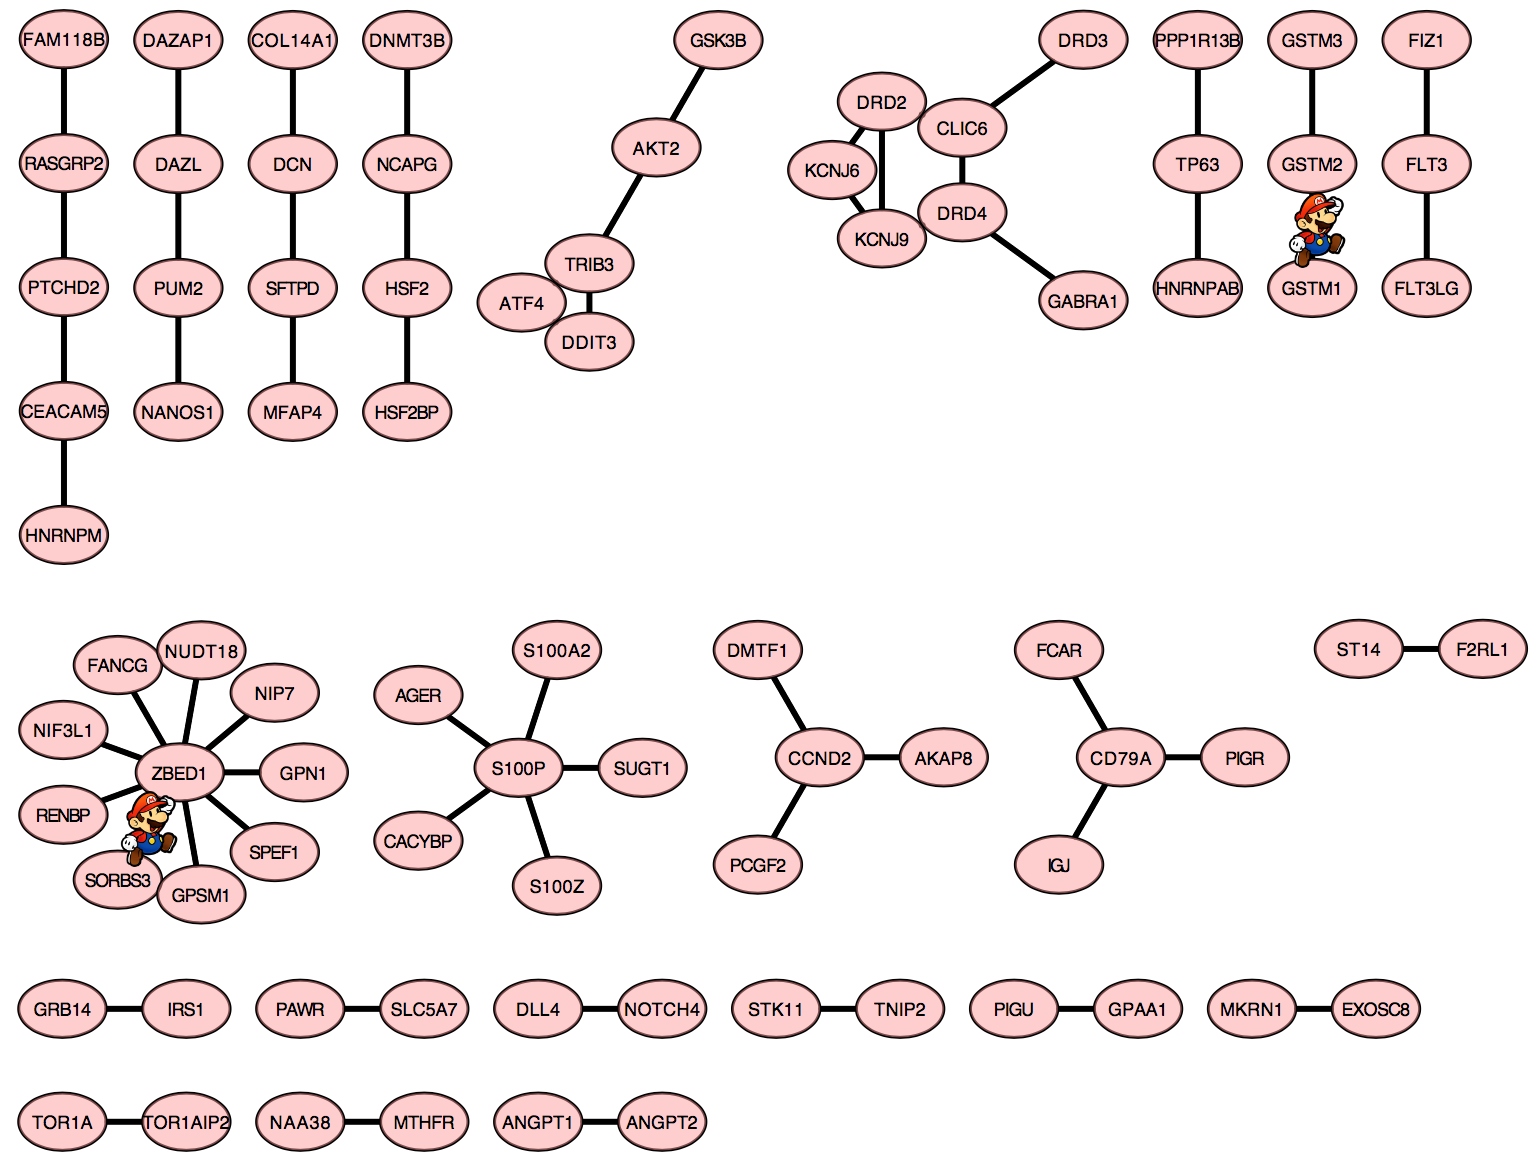
\includegraphics[width=\textwidth]{ch-wavelet/subnetworks_w-analysis_spec}
		\caption{Gene subnetworks identified by the wavelet-analysis method with spectral graph dual wavelets ($82$ genes connected out of $109$ selected).}
		\label{fig3:wanalysis}
	\end{subfigure}
	\caption{Gene subnetworks related to breast cancer survival identified by regularization methods using the METABRIC data and HPRD PPI network.}
	\label{fig3:subnetworks}
\end{figure}






It is interesting to investigate from a biological point of view the genes selected by our survival analysis for breast cancer using the METABRIC gene expression data and the HPRD PPI network, where the regularization parameter $\lambda$ and thus the number of genes selected is determined by cross-validation. In particular, we focus on comparing the three methods denoted by ``e-net'', ``laplasso (norm)'' and ``\wanaspec{}'' for the reminder of the section, each representing a class of methods. The network-free elastic net identified a total of $112$ genes, among which only $10$ genes are not isolated from one another on the HPRD PPI network that form $5$ connected gene pairs (Figure \ref{fig3:enet}). The network-based Laplacian lasso identified a total of $100$ genes, among which $10$ genes are connected and they coincide exactly with the the connected genes identified by the elastic net (Figure \ref{fig3:enet}). Our network-based wavelet-analysis method with spectral graph dual wavelets identified a total of $109$ genes, among which $82$ genes are connected that form $23$ gene modules of various sizes and shapes (Figure \ref{fig3:wanalysis}). We refer to the online supplements for the full list of genes selected by each method and in this study focus on the connected genes that form collaboratively functional gene modules.







The wavelet-based method is able to select more genes that form larger subnetworks than the other two methods. Specifically, there are two pairs of connected genes that are commonly selected by the three methods. First, while the other two methods detected the relation to cancer survival of GSTM2 and GSTM3 genes, the wavelet-based method was able to detect the involvement of three genes from the same gene family that are GSTM1, GSTM2 and GSTM3. In fact, glutathione metabolism is able to play both protective and pathogenic roles with respect to cancer \cite{Balendiran2004role,Wu2004Glutathione}, and the human GSTM gene family encodes the mu class of metabolic isoenzymes of glutathione S-transferase, consisting of five different but closely related isotypes GSTM1 to GSTM5. It has been reported that certain GSTM genes are correlated with the likelihood of breast cancer recurrence and functionally contribute prognostic information \cite{Kiefer2014Multiple}. In particular, GSTM1, which was detected only by the wavelet-based method, has been extensively studied in breast cancer risk especially due to its null genotype \cite{Roodi2004Association,Sull2004Glutathione}, but the absence of a functional GSTM1 enzyme in a null variant can be meaningfully compensated for by GSTM2 \cite{Bhattacharjee2013Functional}. Second, while the other two methods selected ZBED1 and SORBS3 genes simultaneously, the wavelet-based method detected through interactions documented in HPRD a star-shaped subnetwork in which the hub gene ZBED1 is centered around by $9$ other genes SORBS3, FANCG, GPSM1, NUDT18, SPEF1, NIP7, GPN1, RENBP, NIF3L1. This is in fact the largest subnetwork identified by the wavelet-based method, in which some genes are of particular interest. In fact, the ZBED1 gene encodes a protein which binds to DNA elements found in the promoter regions of a number of genes related to cell proliferation \cite{Matsukage2008DREDREF,Yamashita2007hDREF}. The FANCG gene,, which was detected only by the wavelet-based method, provides instructions for making a protein complex involved in the Fanconi anemia (FA) pathway responsible for DNA repair and it has been reported to directly interact with BRCA2 gene that plays an important role in homologous recombination repair and survival risk in breast cancer \cite{Hussain2003Direct,Wilson2008FANCG}.









Among the subnetworks identified exclusively by our wavelet-based method, some are of particular interest and the involvement of the connected genes in cancer biology was previously reported in literature. For example, an interesting subnetwork is composed of $7$ genes DRD2, DRD3, DRD4, CLIC6, KCNJ6, KCNJ9, GABRA1. In fact, the D2-like family of the dopamine receptors, encoded by genes DRD2, DRD3 and DRD4, are coupled to certain guanine nucleotide-binding proteins (G proteins) which directly inhibits adenylate cyclase activity and cyclic adenosine monophosphate (cAMP) formation \cite{Neves2002G}, and whose signaling has been linked to cancer progression and cancer risk \cite{Murphy2009Dopamine,Mao2015Dopamine} leading to many preclinical studies on the antitumor effects sought by antagonizing DRD2 signaling \cite{Pornour2015New,Hoeppner2015Dopamine}. Notably, all three genes DRD2, DRD3 and DRD4 are simultaneously selected due to their common interactor gene CLIC6. The second interesting subnetwork of interest is composed of $5$ genes AKT2, ATF4, DDIT3, GSK3B, TRIB3. In this subnetwork, three genes AKT2, ATF4 and DDIT3 are present in the mitogen-activated protein kinase (MAPK) signaling pathway whose relevance to cancer has been profoundly studied and we refer to \cite{Dhillon2007MAP} for an overview; three genes AKT2, ATF4 and GSK3B are found in the PI3K/Akt signaling pathway whose role in breast cancer has been reported in \cite{FresnoVara2004PI3KAkt,Paplomata2014PI3KAKTmTOR} for instance, and two genes AKT2 and GSK3B are included in the KEGG pathways in cancer. The third interesting subnetwork is a star-shaped gene module composed of $4$ genes CCND2, DMTF1, AKAP8, PCGF2. In fact, the hub gene CCND2 encodes cyclin D2, a protein belonging to a highly conserved family of cyclin proteins that control cell progression through regulating cell cycle. There exists an extensive body of literature on the role of D-type cyclins as a biomarker in cancer phenotype and progression, see \cite{Musgrove2011Cyclin} for a recent review. Connected to gene CCND2 is gene DMTF1 which encodes a cyclin D-binding myb-like transcription factor. DMTF1 was known for its tumor suppressive role linked to the regulation of many signaling pathways involving the tumor protein 53 (TP53) as well as CCND1, see \cite{Tian2017From} for a recent review. The last subnetwork worth special mention is the gene triplet of FLT3, FLT3LG and FIZ1, among which two genes FLT3LG and FLT3 are included in the KEGG pathways in cancer. The gene FLT3 encodes a class III receptor tyrosine kinase that regulates hematopoiesis whose role in the pathogenesis of acute myeloid leukemia (AML) in particular has been long recognized \cite{Levis2003FLT3}. Besides, FLT3LG, namely the FLT3 ligand, also plays a role in the immune response, and hence it was investigated in the pursuit of promising immuno-therapy against cancer by means of vaccine adjuvant \cite{Lynch1997FLT3,Kreiter2011FLT3}. Notably, gene FLT3 was selected by all three methods under consideration, but its connected gene FLT3LG was selected exclusively by the wavelet-based method.












\section{Discussion}
\label{sec3:discussion}








In the present chapter, we have studied network-based regularization methods under a predictive framework with linear models in order to incorporate relationships between features presumably encoded by a known network, and proposed to use network-based wavelet smoothing in order for subnetwork detection by structured feature selection. Notably, the proposed methods are essentially a class of penalty terms that are readily combined with any loss function appropriately chosen depending on the application in fitting linear models, and path-wise algorithms for solving the underlying optimization problems are straightforwardly available by modifying those solving the standard lasso. Finally, we demonstrated the proposed methods by performing survival analysis for breast cancer using METABRIC gene expression data guided by a PPI network obtained from HPRD. Results show that, compared to several state-of-the-art methods, the wavelet-analysis method with spectral graph dual wavelets, as a representative of wavelet-based methods, was able to improve the efficacy of gene selection in terms of stability, connectivity and interpretability, while achieving competitive performance of survival risk prediction. In particular, the wavelet-based method identified larger subnetworks involving more connected genes, and the relevance of many genes to breast cancer survival have been previously reported by independent studies.











Key insights into the superiority of network-based wavelet smoothing to other network-based regularization methods regarding feature selection lie in the properties of graph wavelets. Recall that graph wavelets are graph vectors that are localized on the graph and fully determined by the local structure of the graph. In particular, the construction of graph wavelets conceals an automated procedure of designating subnetworks whose location, size and shape are inherently specified by the underlying graph wavelets. When any graph vector is decomposed into a linear combination of graph wavelets, we obtain a new representation of the graph vector that are decorrelated and modularized with respect to graph wavelets. The idea of wavelet smoothing originates from seeking for a coefficient vector of the linear model that is sparse in its wavelet representation, and the modularized sparsity of the coefficient vector consequently enables direct identification of subnetworks adapted to optimizing the prediction. Contrariwise, the sparsity-inducing term for feature selection in the Laplacian lasso is a standard lasso term that regards features rather individually, despite that an additional Laplacian term controls the global smoothness of the coefficients and thus encourages features closer on the network to be selected simultaneously. Likewise, the spirit of feature selection for the graph fused lasso is indeed direct identification of subnetworks. This is achieved, however, through an estimate of the coefficient vector that is forced piece-wise constant over the network. Therefore, the identified subnetwork is only data-adaptive but not adapted to the locally irregular structure of the network. Besides, when we expect that the relationships between features conform to the network structure, the compulsory restriction seems suboptimal that all features in each subnetwork should share exactly the same coefficients.











When performing network-based analysis of gene expression data, we highlighted the benefits of using a PPI network to guide gene selection related to breast cancer survival. An important issue is that our knowledge of biology about protein-protein interaction is nonetheless incomplete and the edges of the known biological network can even be subject to errors or misspecifications, especially those pertaining to cancer biology. Future research of pressing need would be to investigate how sensitive the results are to perturbation of the network structure. A potentially helpful trick could be to adapt the network to data by removing edges from the network if the correlation of the expression levels between the two connected genes is very small. Another issue prior to employing network-based analysis is to decide which biological network to use, which in principle depends on domain expertise. In fact, the methods considered in this study, including the wavelet-based methods, can be applied with various biological networks such as signaling or metabolic pathways. However, an open question is to compare the list of selected genes and detected subnetworks when guided by different biological networks or from different databases. Finally, we would like to point out that, despite the findings of this study, the rationale for network-guided genomic data analysis for improving prediction performance of breast cancer survival remains a controversial topic \cite{Staiger2013Current}. Comprehensive studies benchmarking the breast cancer survival analysis with more datasets, networks, regularization methods and prediction tasks, such as those that follow the evaluation pipeline of \cite{Staiger2013Current}, is called for in future research.










For the methods of network-based wavelet smoothing, many variants exist and have been empirically tested in the numerical experiments of this study, raising a few points worth discussion and further investigation. First, we observed distinct performance with respect to which version of graph Laplacian (normalized or non-normalized) is used for the construction of spectral graph wavelets. In fact, there are many theoretical guarantees that favor the normalized Laplacian \cite{Chung1997Spectral} but a debate is ongoing over which version should be used in practice. Despite that we opted for the non-normalized Laplacian by default, we do not conclude definitively on the choice of Laplacian that is better suited for the construction of spectral graph wavelets integrated in network-based wavelet smoothing. Second, this study provides an empirical benchmark comparing the performance of two particular types of graph wavelets, that are spectral graph wavelets and lifting-based graph wavelets. Evidences from all experiments strongly advocate the use of spectral graph wavelets over lifting-based graph wavelets, and the substantially deficient performance of latter is somewhat surprising. In fact, if data are time series that reside on 1-dimensional chain graph, it has been proven that any discrete wavelet transform with all classical wavelet filter banks can be factored into a sequence of lifting steps \cite{Daubechies1998Factoring}. Therefore, it calls for theoretical studies that provide a unifying overview of different techniques of performing wavelet transform on general graphs. Third, we proposed to use two approaches to wavelet smoothing, namely the synthesis approach \eqref{eq3:synthesis} and the analysis approach \eqref{eq3:analysis}. Despite the similarity in their mathematical formulation, the motivation underlying both approaches differ fundamentally. The synthesis approach seeks a reconstruction of the coefficient vector as a sparse combination of graph wavelets, while the analysis approach aspires to build sparse predictive models on the wavelet-transformed feature data. Our real-data experiments on survival analysis for breast cancer particularly suggest that the analysis approach usually outperforms the synthesis approach, as observed also by \cite{Elad2007Analysis}.









There are many interesting extensions of the current work. One direction would be to perform wavelet smoothing on directed graphs or graphs with some edge attributes. This is particularly relevant when we would like to explore relationships between features associated with irreversible direction and meaningful attributes. For example, in a signaling network, each edge is associated with a direction (indicating cell signaling is transduced from one gene to another but cannot be reversed) as well as an annotated type of interaction (activation or inhibition). Another direction would be to explore the possibility of adopting, besides graph wavelet transform, other types of localized or multiscale transforms specifically designed to analyze data on graphs, such as windowed graph Fourier transform \cite{Shuman2012windowed} or multiscale graph pyramid transform \cite{Shuman2016multiscale}. In particular when the two directions engage in one application, deeper understanding of the network utilized can be enlightening for the applicability of the methods and transforms employed.

